% -*- coding: utf-8 -*-

\begin{chapter}{Глубинная циркуляция}\label{chap:13}
% \chapter{Deep Circulation in the Ocean} 
Непосредственное влияние ветра на циркуляцию океана, рассмотренное 
в нескольких предыдущих главах, наиболее сильно проявляется в приповерхностном
слое воды толщиной порядка километра. Ниже этого слоя расположена 
обширная водная масса, простирающаяся до глубины~$4$--$5\km$. Температура
во всем этом объеме воды не превышает~$\degCent{4}$. Формирование данной
водной массы происходит за счет опускания в высоких широтах поверхностной
холодной и плотной воды на большие глубины. Далее эта вода распространяется
в горизонтальном направлении, заполняя океанские котловины. Глубинное
перемешивание\index{перемешивание!глубинных вод} в конечном итоге приводит
к подъему воды через термоклин\index{термоклин!перемешивание в}%
\index{перемешивание!в термоклине} на больших площадях. Этот
подъем воды\index{перемешивание!глубинных слоев} и служит движущей силой
глубинной циркуляции.  
Данные глубины океана принято называть 
\textit{абиссопелагиалью}\index{абиссопелагиаль|textbf}, а циркуляцию,
соответственно, \textit{абиссальной циркуляцией}%
\index{абиссальная циркуляция|textbf}\index{циркуляция!абиссальная|textbf}%
\index{океанская циркуляция!абиссальная|textbf}.
%
% The direct forcing of the oceanic circulation by wind discussed in the
% last few chapters is strongest in the upper kilometer of the water
% column. Below a kilometer lies the vast water masses of the ocean
% extending to depths of 4--5 km.  The water is everywhere cold, with a
% potential temperature less than 4\degrees C.  The water mass is formed
% when cold, dense water sinks from the surface to great depths at high
% latitudes. It spreads out from these regions to fill the ocean
% basins. Deep mixing\index{mixing!of deep waters} eventually pulls the
% water up through the thermocline\index{thermocline!mixing
% in}\index{mixing!in thermocline} over large areas of the ocean. It is
% this upward mixing\index{mixing!of deep waters} that drives the deep
% circulation.  The vast deep ocean is usually referred to as the
% \textit{abyss}\index{abyss|textbf}, and the circulation as the
% \textit{abyssal circulation}\index{abyssal
% circulation|textbf}\index{circulation!abyssal|textbf}\index{oceanic
% circulation!abyssal|textbf}.

Наиболее плотные поверхностные воды, плотность которых достаточно велика,
чтобы погрузиться до самого дна, формируются в Атлантическом океане между
Норвегией и Гренландией, а также возле Антарктиды под воздействием холодных 
ветров, дующих над океаном в высоких широтах в зимний период. Ветер охлаждает
воду и способствует ее испарению. При достаточно низкой температуре воздуха
образуется морской лед, увеличивая солёность воды за счет вымораживания.
Придонная вода\index{придонная вода!Североатлантическая} формируется 
исключительно в этих двух регионах. Холодные плотные воды также образуются 
в северной части Тихого океана, но их солёность недостаточна для проникновения 
до самого дна.
%
% The densest water at the sea surface, water that is dense enough to
% sink to the bottom, is formed when frigid air blows across the ocean
% at high latitudes in winter in the Atlantic between Norway and
% Greenland and near Antarctica. The wind cools and evaporates water. If
% the wind is cold enough, sea ice forms, further increasing the
% salinity of the water because ice is fresher than sea water.  Bottom
% water\index{bottom water!North Atlantic} is produced only in these two
% regions. Cold, dense water is formed in the North Pacific, but it is
% not salty enough to sink to the bottom.

С другой стороны, в средних и низких широтах плотность воды даже в зимний
период существенно меньше, так что эта вода не может опуститься глубже
нескольких сотен метров. Исключение составляют некоторые моря, например,
Средиземное, испарение в которых столь велико, что плотность воды оказывается
достаточной для погружения на дно этих морей. Если существует возможность
обмена водами с открытым океаном, происходит перемешивание вод, сформированных
в морях в зимний период, с водами океана, после чего они распространяются
в океане на средних глубинах.
%
% At mid and low latitudes, the density, even in winter, is sufficiently
% low that the water cannot sink more than a few hundred meters into the
% ocean. The only exception are some seas, such as the Mediterranean
% Sea, where evaporation is so great that the salinity of the water is
% sufficiently great for the water to sink to the bottom of these
% seas. If these seas can exchange water with the open ocean, the waters
% formed in winter in the seas mixes with the water in the open ocean
% and it spreads out along intermediate depths in the open ocean.


\begin{section}{Определение понятия глубинной циркуляции}
% \section{Defining the Deep Circulation}
Для описания глубинной циркуляции было введено большое количество терминов, 
в том числе:
1) \emph{абиссальная циркуляция}\index{абиссальная циркуляция}%
\index{циркуляция!абиссальная}\index{океанская циркуляция!абиссальная}, 
2) \emph{термохалинная циркуляция}, 
3) \emph{меридиональная опрокидывающая циркуляция}%
\index{циркуляция!меридиональная опрокидывающая|textbf}%
\index{океанская циркуляция!меридиональная опрокидывающая|textbf}%
\remark{Термин <<меридиональная опрокидывающая циркуляция>> встречается
в некоторых русскоязычных публикациях IPCC 
(\href{http://www.ipcc.ch/pdf/assessment-report/ar4/wg1/ar4-wg1-annex-ru.pdf}%
{\url{http://www.ipcc.ch/pdf/assessment-report/ar4/wg1/ar4-wg1-annex-ru.pdf}}),
но наряду с этим в других источниках также используется термин 
\emph{меридиональная термохалинная циркуляция}.}
и 4) \emph{глобальный конвейер}. 
Термин <<термохалинная циркуляция>> получил в свое время широкое 
распространение, но в дальнейшем практически исчез из океанологической
литературы (Toggweiler and Russell, 2008). Причиной этого считается как
появление новых данных, из которых следует, что плотность не влияет
на характер движения потоков, так и отсутствие ясного определения самой
концепции (Wunsch, 2002b).
%
% Many terms have been used to describe the deep circulation. They
% include: 1) \textit{abyssal circulation}\index{abyssal circulation}%
% \index{circulation!abyssal}\index{oceanic circulation!abyssal}, 2)
% \textit{thermohaline circulation} 3) \textit{meridional overturning
% circulation}\index{circulation!meridional
% overturning|textbf}\index{oceaniccirculation!Meridional
% Overturning|textbf}, and 4) \textit{global conveyor}.  The term
% thermohaline circulation was once widely used, but it has almost
% entirely disappeared from the oceanographic literature (Toggweiler and
% Russell, 2008). It is no longer used because it is now clear that the
% flow is not density driven, and because the concept has not been
% clearly defined (Wunsch, 2002b).

Понятие меридиональной опрокидывающей циркуляции определено значительно лучше. 
Она представляет собой зональное среднее потока как функцию глубины и широты.
Графики циркуляции показывают области, в которых вертикальные потоки играют
важную роль, но по ним невозможно установить влияние на поток океанских
круговоротов.
%
% The meridional overturning circulation is better defined. It is the
% zonal average of the flow plotted as a function of depth and
% latitude. Plots of the circulation show where vertical flow is
% important, but they show no information about how circulation in the
% gyres influences the flow.

Следуя работе Вюнша (Wunsch, 2002b), будем считать глубинную циркуляцию
переносом массы. Безусловно, циркуляция массы также переносит тепло, соли,
кислород и т.п., но перенос таких характеристик может отличаться
от переноса массы\index{перенос!массы}. Например, как указывает Вюнш,
в северной части Атлантического океана происходит приток тепла и отток 
кислорода.
%
% Following Wunsch (2002b), I define the deep circulation as the
% circulation of mass. Of course, the mass circulation also carries
% heat, salt, oxygen, and other properties. But the circulation of the
% other properties is not the same as the mass
% transport\index{transport!mass}. For example, Wunsch points out that
% the north Atlantic imports heat but exports oxygen.
\end{section}
 
\begin{section}{Важность глубинной циркуляции}
% \section{Importance of the Deep Circulation}
\index{глубинная циркуляция!важность}\index{циркуляция!глубинная!важность}%
\index{океанская циркуляция!глубинная!важность}%
Глубинная циркуляция обеспечивает глобальный перенос тепла, солей, 
кислорода, \COtwo{} и~пр.\ из области высоких широт в низкие в зимний 
период. Благодаря этому явлению имеют место следующие важные последствия:
%
% \index{deep circulation!importance
% of}\index{circulation!deep!importance of}\index{oceanic
% circulation!deep!importance of}The deep circulation carries heat,
% salinity, oxygen, CO$_2$, and other properties from high latitudes in
% winter to lower latitudes throughout the world. This has very
% important consequences.

\begin{enumerate}
\item 
Температурный контраст между холодными глубинными и теплыми поверхностными
водами определяет стратификацию океана, которая существенно влияет на его
динамику.
%
% \vitem The contrast between the cold deep water and the warm surface
% waters determines the stratification of the ocean, which strongly
% influences ocean dynamics.

\item 
Объем глубинных вод существенно превышает объем поверхностных. Несмотря
на то, что глубинные течения сравнительно слабы, величина их 
переноса\index{перенос!объем, глубинный} сравнима с поверхностным.
%
% \vitem The volume of deep water is far larger than the volume of
% surface water. Although currents in the deep ocean are relatively
% weak, they have transports\index{transport!volume, in deep ocean}
% comparable to the surface transports.

\item 
Потоки тепла и другие параметры глубинной циркуляции воздействуют на тепловой
баланс Земли и климат. Изменчивость потоков может иметь различные временные
масштабы, от десятилетий до тысячелетий, и эта изменчивость влияет на климат
в указанных временных промежутках. Океан может быть основной причиной
изменчивости длительностью от нескольких лет до десятилетий, а также он
мог оказывать влияние на климат во время ледниковых периодов.
%
% \vitem The fluxes of heat and other variables carried by the deep
% circulation influences earth's heat budget and climate. The fluxes
% vary from decades to centuries to millennia, and this variability
% modulates climate over such time intervals. The ocean may be the
% primary cause of variability over times ranging from years to decades,
% and it may have helped modulate ice-age climate.
\end{enumerate}
Два аспекта глубинной циркуляции особенно важны для понимания земного климата
и его возможной реакции на увеличение концентрации углекислого 
газа~\COtwo{} в атмосфере: i) способность холодной воды поглощать
и удерживать атмосферные~\COtwo{} и тепло; ii) способность глубинных
течений регулировать величину переноса тепла\index{перенос!тепла} 
из тропиков в высокие широты.
%
% Two aspects of the deep circulation are especially important for
% understanding earth's climate and its possible response to increased
% carbon dioxide CO$_2$ in the atmosphere: i) the ability of cold water
% to store CO$_2$ and heat absorbed from the atmosphere, and ii) the
% ability of deep currents to modulate the heat
% transported\index{transport!heat} from the tropics to high latitudes.

\begin{paragraph}{Океан как вместилище углекислоты.}
% \paragraph{The ocean as a Reservoir of Carbon Dioxide}
\index{углекислота}Океан является основным вместилищем свободного углекислого
газа~\COtwo{}, играющего важную роль в механизме парникового эффекта. 
В океане содержится $40\,000~\GtC$ (растворенного, взвешенного, 
и входящего в состав живых организмов), 
на суше~--- $2\,200\GtC$, а в атмосфере~--- всего лишь~$750\GtC$. 
Следовательно, содержание углерода в океане превышает 
атмосферное в 50~раз. Более того, количество нового углерода, поступившего
в атмосферу с начала промышленной революции, $150\GtC$, меньше количества
углерода, проходящего через морскую экосистему в течение 5~лет.
($1\GtC = 1\text{~гигатонна углерода} = 10^{12}\kg$ углерода.) 
Еще больший объем углерода входит в состав карбонатных пород,
таких как известняк, раковин морских животных, кораллов и т.п. 
Однако, этот углерод связан, и его участие в обмене с другими вместилищами 
углерода затруднено.
%
% \index{carbon dioxide}The ocean are the primary reservoir of readily
% available CO$_2$, an important greenhouse gas. The ocean contain
% 40,000 GtC of dissolved, particulate, and living forms of carbon. The
% land contains 2,200 GtC, and the atmosphere contains only 750
% GtC. Thus the ocean hold 50 times more carbon than the
% air. Furthermore, the amount of new carbon put into the atmosphere
% since the industrial revolution, 150 GtC, is less than the amount of
% carbon cycled through the marine ecosystem in five years. (1 GtC = 1
% gigaton of carbon = $10^{12}$ kilograms of carbon.) Carbonate rocks
% such as limestone, the shells of marine animals, and coral are other,
% much larger, reservoirs. But this carbon is locked up. It cannot be
% easily exchanged with carbon in other reservoirs.

Растворимость~\COtwo{} в холодной воде выше, чем в теплой. Представьте
себе, что случится, если потрясти, а затем открыть бутылку теплой 
газированной воды. Выделение~\COtwo{} из теплой воды будет происходить
гораздо быстрее, чем из холодной. Следовательно, основным вместилищем
растворенного в океане \COtwo{} служат холодные глубинные воды.
%
% More CO$_2$ dissolves in cold water than in warm water. Just imagine
% shaking and opening a hot can of Coke$^{\mbox{\textsf{\scriptsize
% TM}}}$. The CO$_2$ from a hot can will spew out far faster than from a
% cold can. Thus the cold deep water in the ocean is the major reservoir
% of dissolved CO$_2$ in the ocean.

Количество свободного~\COtwo{} в атмосфере увеличивается за счет
сжигания ископаемого топлива и древесины. В течение короткого промежутка
времени $48\%$ вновь поступившего в атмосферу~\COtwo{} растворяется в 
океане (Sabine et al, 2004), при этом большая часть растворенной углекислоты
оказывается в конечном итоге в глубинах океана.
%
% New CO$_ 2$ is released into the atmosphere when fossil fuels and
% trees are burned. Very quickly, 48\% of the CO$_2$ released into the
% atmosphere dissolves into the ocean (Sabine et al, 2004), much of
% which ends up deep in the ocean.

Прогнозирование изменений климата существенно зависит от количества
поглощенного~\COtwo{} и продолжительности его нахождения в океане. Если эти
величины невелики, концентрация углекислого газа в атмосфере будет изменяться, 
воздействуя на длинноволновый радиационный баланс. Объем растворенного в 
океане~\COtwo{} и длительность его пребывания там зависят от величины
переноса\index{перенос!углекислоты}~\COtwo{} глубинной циркуляцией и от
суммарного потока углерода, откладывающегося на дне океана. 
Количество растворенной углекислоты зависит от температуры глубинной воды,
продолжительность нахождения в глубоких слоях~--- от скорости их обновления,
а величина отложений~--- от того, подверглись ли окислению останки животных 
и растений, опускающиеся на морское дно. Усиление вентиляции глубинных слоев 
и их нагрев могут привести к выбросу большого количества углекислоты 
в атмосферу.
%
% Forecasts of future climate change depend strongly on how much CO$_2$
% is stored in the ocean and for how long. If little is stored, or if it
% is stored and later released into the atmosphere, the concentration in
% the atmosphere will change, modulating earth's long-wave radiation
% balance. How much and how long CO$_2$ is stored in the ocean depends
% on the transport\index{transport!carbon dioxide} of CO$_2$ by the deep
% circulation and on the net flux of carbon deposited on the sea
% floor. The amount that dissolves depends on the temperature of the
% deep water, the storage time in the deep ocean depends on the rate at
% which deep water is replenished, and the deposition depends on whether
% the dead plants and animals that drop to the sea floor are oxidized.
% Increased ventilation of deep layers, and warming of the deep layers
% could release large quantities of the gas to the atmosphere.

Накопление углерода в океане также зависит от динамики морских экосистем,
апвеллинга\index{апвеллинг!и накопление углерода} и количества органических 
останков, накапливающихся в донных отложениях. Однако, мы не будем 
рассматривать вопрос столь подробно.
%
% The storage of carbon in the ocean also depends on the dynamics of
% marine ecosystems, upwelling\index{upwelling!and carbon storage}, and
% the amount of dead plants and animals stored in sediments. But I won't
% consider these processes.
\end{paragraph}

\begin{paragraph}{Перенос тепла океаном.}
% \paragraph{Oceanic Transport of Heat}
\index{перенос тепла!океанический}\index{перенос!тепла}Океан переносит
из тропиков примерно половину всего тепла, необходимого для поддержания
существующей температуры на поверхности Земли. Благодаря переносу тепла 
Гольфстримом\index{Гольфстрим!перенос тепла} и Северо-Атлантическим течением
северная часть Атлантического океана свободна от льда, а климат Европы
мягче. Так, в Норвегии, лежащей под~\latlon{60}{N}, гораздо теплее, чем
на юге Гренландии либо в северной части Лабрадора, несмотря на их 
расположение на той же широте. На западном побережье Ирландии растут
пальмы, но их нет на Ньюфаундленде, расположенном южнее.
%
% \index{heat transport!oceanic}\index{transport!heat}The ocean carry
% about half the heat out of the tropics needed to maintain earth's
% temperature. Heat carried by the Gulf Stream\index{Gulf
% Stream!transport of heat by} and the north Atlantic drift keeps the
% far north Atlantic ice free, and it helps warm Europe. Norway, at
% 60\degrees N is far warmer than southern Greenland or northern
% Labrador at the same latitude. Palm trees grow on the west coast of
% Ireland, but not in Newfoundland which is further south.

Уоллес Брокер (Геофизическая обсерватория Ламон-Доэрти, Колумбийский 
университет), называет океанский компонент системы переноса 
тепла\index{перенос!тепла} \emph{Глобальным конвейером}%
\index{Глобальный конвейер}\index{перенос тепла!Глобальный конвейер} 
(Wally Broecker, 1987). Суть его теории в том, что поверхностные течения
переносят тепло в отдаленную северную часть Атлантического океана 
(рис.~\ref{fig:fig13-1}). Там поверхностные воды отдают тепло и влагу 
атмосфере, после чего становятся достаточно холодными, солёными и плотными,
чтобы погрузиться до самого дна\index{придонная вода!Североатлантическая} 
в Норвежском и Гренландском морях. Далее эта вода переносится холодными 
придонными течениями южнее. Часть воды остается на поверхности и возвращается
на юг холодными поверхностными течениями, например, Лабрадорским 
и Португальским (рис.~\ref{fig:NATLcur1}). Очень хороший обзор наших знаний
о глобальном конвейере был опубликован Ричардсоном (Richardson, 2008).
%
% Wally Broecker (1987), working at Lamont-Doherty Geophysical
% Observatory of Columbia University, calls the oceanic component of the
% heat-transport\index{transport!heat} system the \textit{Global
% Conveyor Belt}\index{Global Conveyer Belt}\index{heat transport!Global
% Conveyer Belt}. The basic idea is that surface currents carry heat to
% the far north Atlantic (figure 13.1). There the surface water releases
% heat and water to the atmosphere, and it becomes sufficiently cold,
% salty, and dense that it sinks to the bottom\index{bottom water!North
% Atlantic} in the Norwegian and Greenland Seas. It then flows southward
% in cold, bottom currents. Some of the water remains on the surface and
% returns to the south in cool surface currents such as the Labrador
% Current and Portugal Current (see figure 11.8). Richardson (2008) has
% written a very useful paper surveying our understanding of the global
% conveyor belt.

Придонная вода из северной части Атлантического 
океана\index{придонная вода!Североатлантическая} is mixed upward 
в других регионах and ocean, благодаря чему в конечном итоге возвращается
обратно в Гольфстрим и северную Атлантику. Таким образом, большая часть воды,
погружающейся на дно в северной части Атлантического океана, должна заменяться
водой из более южных его регионов. По мере продвижения этой поверхностной воды
в северном направлении через экватор и далее в Гольфстрим, она переносит
с собой тепло из южной Атлантики.
%
% The deep bottom water from the north Atlantic\index{bottom water!North
% Atlantic} is mixed upward in other regions and ocean, and eventually
% it makes its way back to the Gulf Stream and the North Atlantic. Thus
% most of the water that sinks in the north Atlantic must be replaced by
% water from the far south Atlantic. As this surface water moves
% northward across the equator and eventually into the Gulf Stream, it
% carries heat out of the south Atlantic.

Величина переноса тепла\index{перенос!тепла} в северном направлении в ходе
образования Североатлантической придонной воды в зимний период столь велико,
что суммарный перенос тепла в Атлантическом океане в целом направлен к северу
даже в южном полушарии (рис.~\ref{fig:heattransport}). Большая часть солнечного
тепла, поглощенного Атлантическим океаном в тропиках, переносится на север
и обогревает Европу и северное полушарие в целом. Представьте себе, что может
произойти, если бы этот перенос тепла прекратился. Мы рассмотрим данный вопрос
в следующем разделе.
%
% So much heat is pulled\index{transport!heat} northward by the
% formation of north Atlantic bottom water in winter that heat transport
% in the Atlantic is entirely northward, even in the southern hemisphere
% (figure 5.11). Much of the solar heat absorbed by the tropical
% Atlantic is shipped north to warm Europe and the northern
% hemisphere. Imagine then what might happen if the supply of heat is
% shut off. I will get back to that topic in the next section.

\begin{figure}[t!]
\makebox[120mm] [c]{\includegraphics{pics/fig13-1}} 
\caption{Поверхностные (узкая штриховая линия) и глубинные (широкая)
течения в северной части Атлантического океана. Северо-Атлантическое
течение переносит теплую воду к северу, где она охлаждается. Некоторое 
количество воды погружается и возвращается обратно на юг благодаря глубинным
западным пограничным течениям, а другая ее часть~--- по поверхности. 
(По данным Вудсхолского института океанологии.)}
\label{fig:fig13-1}
\end{figure}
%
% \begin{figure}[t!]
% \makebox[120mm] [c]{\includegraphics{fig13-1}}
% \footnotesize
% Figure 13.1 The surface (narrow dashes) \rule{0mm}{3ex}and deep (wide
% dashes) currents in the north Atlantic. The North Atlantic Current
% brings warm water northward where it cools.  Some sinks and returns
% southward as a cold, deep, western-boundary current. Some returns
% southward at the surface. From Woods Hole Oceanographic Institution.
% \label{fig:fig13-1}
% \vspace{-4ex}
% \end{figure}

Попробуем грубо оценить важность поверхностной и глубинной циркуляции в 
северной части Атлантического океана при помощи вычислений на основе 
информации о водах Атлантического океана, обобщенной Биллом Шмитцем в 
замечательной работе (Bill Schmitz, 1996), подводящей итог всей его научной
деятельности. Гольфстрим\index{Гольфстрим!перенос} 
переносит\index{перенос!Гольфстрима} $40\Sv$ воды с температурой~$\degCent{18}$
к северу. Этот перенос частично компенсируется переносом~$14\Sv$ воды
к югу глубинным западным пограничным течением при температуре~$\degCent{2}$. 
Таким образом, вода должна отдать~$0.9\Pwt$ ($1\Pwt = 10^{15}\wt$)
в северной части Атлантического океана выше \latlon{24}{N} 
Несмотря на то, что данные вычисления крайне грубы, они весьма близки
к величине~$1.2\,\pm\,0.2\Pwt$, полученной в результате более тщательной
оценки, выполненной Rintoul и Вюншем (Rintoul and Wunsch, 1991).
%
% We can make a crude estimate of the importance of the north Atlantic
% surface and deep circulation from a calculation based on what we know
% about waters in the Atlantic compiled by Bill Schmitz (1996) in his
% wonderful summary of his life's work. The Gulf Stream\index{Gulf
% Stream!transport} carries\index{transport!by Gulf Stream} 40 Sv of
% 18\degrees C water northward. Of this, 14 Sv return southward in the
% deep western boundary current at a temperature of 2\degrees C. The
% water must therefore lose 0.9 petawatts (1 petawatt $= 10^{15} $ watt)
% in the north Atlantic north of 24\degrees N. Although the calculation
% is very crude, it is remarkably close to the value of $1.2\,\pm\,0.2$
% petawatts estimated much more carefully by Rintoul and Wunsch (1991).

Отметим, что если бы вода оставалась на поверхности и возвращалась обратно
в виде восточного пограничного течения, она бы вернулась на юг гораздо более
теплой, чем в случае глубинного течения. Следовательно, перенос 
тепла\index{перенос!тепла} при этом был бы существенно меньше и, возможно,
оказался бы недостаточным для поддержания северной части Атлантического океана
свободной от льда. 
%
% Note that if the water remained on the surface and returned as an
% eastern boundary current, it would be far warmer than the deep current
% when it returned southward. Hence, the heat
% transport\index{transport!heat} would be much reduced and it would
% probably not keep the far north Atlantic ice free.

Процесс формирования придонной воды\index{придонная вода} находится под
влиянием поверхностной солёности и ветров в северной Атлантике 
(Toggweiler and Russell, 2008). Он также зависит от скорости 
апвеллинга\index{апвеллинга}, происходящего благодаря 
перемешиванию\index{перемешивание!глубинных вод} в других регионах океана.
Рассмотрим для начала влияние солёности.
%
% The production of bottom water\index{bottom water} is influenced by
% the surface salinity and winds in the north Atlantic (Toggweiler and
% Russell, 2008). It is also influenced by the rate of
% upwelling\index{upwelling} due to mixing\index{mixing!of deep waters}
% in other oceanic areas. First, let's look at the influence of
% salinity.

Более солёные поверхностные воды в зимний период приобретают большую плотность,
чем воды с меньшей солёностью. На первый взгляд, температура представляется
не менее важным фактором, но в высоких широтах вода во всех океанах достигает
температуры замерзания, так что температура воды на поверхности 
составляет~$\degCent{-2}$. При этом в состоянии погрузиться оказывается лишь 
вода с наибольшей солёностью, которая встречается в Атлантическом океане
и подо льдом в области континентального шельфа Антарктиды.
%
% Saltier surface waters form denser water in winter than less salty
% water. At first you may think that temperature is also important, but
% at high latitudes water in all ocean basins gets cold enough to
% freeze, so all ocean produce $-2$\degrees C water at the surface. Of
% this, only the most salty will sink, and the saltiest water is in the
% Atlantic and under the ice on the continental shelves around
% Antarctica.

Процесс формирования придонной воды особо чувствителен к небольшим изменениям
солёности. Так, Рамшторф показал на основе численных моделей меридиональной
опрокидывающей циркуляции\index{циркуляция!меридиональная опрокидывающая}, 
что изменчивость потока пресной воды в северной части Атлантического
океана порядка~$\pm 0.1\Sv$ может как вызывать, так и прекращать глубинную
циркуляцию величиной в~$14\Sv$ (Rahmstorf, 1995). Если формирование придонной
воды во временном промежутке, характеризуемом низкой солёностью, прекратится,
вместе с этим может прекратиться и перенос $1\Pwt$~тепла. 
Weaver и Hillaire-Marcel указывают, что вероятность подобного события низка, 
и если даже оно и произойдет, его последствием будет изменение европейского 
климата в сторону охлаждения, но вовсе не наступление нового ледникового 
периода, благодаря сегодняшней более высокой концентрации~\COtwo{} в атмосфере
(Weaver and Hillaire-Marcel, 2004).
%
% The production of bottom water is remarkably sensitive to small
% changes in salinity. Rahmstorf (1995), using a numerical model of the
% meridional over\-turning circulation\index{circulation!meridional
% overturning}, showed that a $\pm$0.1Sv variation of the flow of fresh
% water into the north Atlantic can switch on or off the deep
% circulation of 14 Sv. If the deep-water production is shut off during
% times of low salinity, the 1 petawatt of heat may also be shut
% off. Weaver and Hillaire-Marcel (2004) point out that the shutdown of
% the production of bottom water is unlikely, and if it did happen, it
% would lead to a colder Europe, not a new ice age, because of the
% higher concentrations of CO$_2$ now in the atmosphere.

Обратим внимание, что выше было сказано:
\emph{<<может прекратиться>>},--- поскольку океан~--- очень сложная система.
На данный момент мы не располагаем какими-либо сведениями о возможном 
увеличении переноса тепла\index{перенос!тепла} другими процессами в случае 
нарушения глубинной циркуляции. Например, циркуляция на средних глубинах 
может усилиться при ослаблении глубинной.
%
% I write \textit{may be shut off} because the ocean is a very complex
% system. We don't know if other processes will increase heat
% transport\index{transport!heat} if the deep circulation is
% disturbed. For example, the circulation at intermediate depths may
% increase when deep circulation is reduced.

Формирование придонной воды также особо чувствительно к небольшим изменениям
в процессах глубинного перемешивания\index{перемешивание!глубинное}. 
Манк и Вюнш вычислили, что для приведения в действие механизма глубинной
циркуляции требуется~$2.1\Twt$ ($1\Twt = 10^{12}\wt$), и что этот
небольшой источник механического 
перемешивания\index{перемешивание!и поток тепла к полюсу} приводит в движение
направленный к полюсу поток тепла\index{тепла поток!к полюсу} 
величиной~$2000\Twt$ (Munk and Wunsch, 1998). 
Некоторая часть энергии перемешивания\index{перемешивание!энергия} сообщается
ветрами, которые могут вызывать в океане турбулентное 
перемешивание\index{перемешивание!ветровое}. Также энергия может высвобождаться
во время диссипации приливных течений\index{перемешивание!приливное}, 
которые зависят от расположения континентов. Наконец, источником энергии
служат глубинные потоки воды через систему срединно-океанических хребтов.
Следовательно, во время последнего ледникового периода, когда уровень моря был
существенно ниже, все упомянутые явления: приливы, приливные течения,
диссипация приливов, ветры и глубинная циркуляция~--- существенно отличались
по своим параметрам от современных.
%
% The production of bottom water is also remarkably sensitive to small
% changes in mixing\index{mixing!of deep waters} in the deep ocean. Munk
% and Wunsch (1998) calculate that 2.1 TW (terawatts $= 10^{12}$ watts)
% are required to drive the deep circulation, and that this small source
% of mechanical mixing\index{mixing!and poleward heat flux} drives a
% poleward heat flux\index{heat flux!poleward} of 2000 TW. Some of the
% energy for mixing\index{mixing!energy for} comes from winds which can
% produce turbulent mixing\index{mixing!by winds} throughout the
% ocean. Some energy comes from the dissipation of tidal
% currents\index{mixing!tidal}, which depend on the distribution of the
% continents. Some of the energy comes from the flow of deep water past
% the mid-ocean ridge system. Thus during the last ice age, when sea
% level was much lower, tides, tidal currents, tidal dissipation, winds,
% and deep circulation all differed from present values.
\end{paragraph}

\begin{paragraph}{Роль океана в климатических флуктуациях ледникового периода.}
% \paragraph{Role of the Ocean in Ice-Age Climate Fluctuations}
\index{ледниковый период|(}Что может произойти, если процесс образования
придонной воды в северной части Атлантического океана остановится? 
Важную информацию об этом можно почерпнуть из ледяного покрова Гренландии
и Антарктиды, а также осадочного слоя в северной Атлантике и озерах.
%
% \index{ice-age|(}What might happen if the production of deep water in
% the Atlantic is shut off? Information contained in Greenland and
% Antarctic ice sheets, in north Atlantic sediments, and in lake
% sediments provide important clues.

Некоторые ледяные керны, полученные в Гренландии и Антарктиде, представляют
собой непрерывную картину атмосферных 
условий\index{атмосферные условия!исторические} в данных регионах на протяжении
до~$700\,000$~лет. Возраст отложений определяется подсчетом годичных слоев.
По мере приближения к более давним слоям, они становятся все хуже различимы,
так что датировка производится по глубине залегания слоя и по слоям пыли
хорошо датированных вулканических извержений. Соотношение изотопов кислорода
во льду позволяет определить температуру воздуха на поверхности ледника во
время формирования льда. Концентрация дейтерия дает температуру поверхности
океана в регионе происхождения влаги. Пузырьки воздуха, заключенные во льду,
содержат данные о концентрации в атмосфере~\COtwo{} и метана.
Пыльца растений, chemical composition и твердые частицы дают информацию 
о вулканических извержениях, скорости и направлении ветров. 
Толщина годичных слоев соответствует скорости снегонакопления. 
Наконец, изотопы некоторых элементов позволяют определить
солнечную активность и интенсивность космического излучения (Alley, 2000).
%
% Several ice cores through the Greenland and Antarctic ice sheets
% provide a continuous record of atmospheric
% conditions\index{atmospheric conditions!finding historical} over
% Greenland and Antarctica extending back more than 700,000 years before
% the present in some cores. Annual layers in the core are counted to
% get age. Deeper in the core, where annual layers are hard to see, age
% is calculated from depth and from dust layers from well-dated volcanic
% eruptions. Oxygen-isotope ratios of the ice give air temperature at
% the glacier surface when the ice was formed. Deuterium concentrations
% give ocean-surface temperature at the moisture source region. Bubbles
% in the ice give atmospheric CO$_2$ and methane concentration. Pollen,
% chemical composition, and particles give information about volcanic
% eruptions, wind speed, and direction. Thickness of annual layers gives
% snow accumulation rates. And isotopes of some elements give solar and
% cosmic ray activity (Alley, 2000).

Керны донных осадочных слоев, полученные в Северной Атлантике в рамках
Ocean Drilling Program, содержат важную информацию о i) поверхностных
и глубинных температуре и солености водяного столба над местом взятия пробы,
ii) формировании североатлантической придонной воды, 
iii) объеме ледников,
и iv) образовании айсбергов. 
Вместе ледяные и осадочные керны позволили провести реконструкцию климата
на протяжении последних нескольких сотен тысяч лет.
%
% Cores through deep-sea sediments in the north Atlantic made by the
% Ocean Drilling Program give information about i) surface and deep
% temperatures and salinity at the location of above the core, ii) the
% production of north Atlantic deep water, iii) ice volume in glaciers,
% and iv) production of icebergs. Ice-sheet and deep-sea cores have
% allowed reconstructions of climate for the past few hundred thousand
% years.

\begin{enumerate}
\item 
Данные о содержании в кернах изотопов кислорода и дейтерия указывают на
многочисленные резкие изменения климата на протяжении последних 
$700\,000\yrs$. В последнем ледниковом периоде температура в
районе Гренландии множество раз быстро возрастала в течение $1$--$100\yrs$,
после чего следовал более долгий период последовательного охлаждения
(Dansgaard et al, 1993). Например, около $11\,500\yrs$~назад
температура в Гренландии повысилась примерно на~$\degCent{8}$ 
в течение $40\yrs$ за три этапа, каждый из которых 
продолжался~$5\yrs$ (Alley, 2000). Такое внезапное потепление называется
\emph{событием (или осцилляцией) Дансгора-Эшгера}%
\index{Дансгора-Эшгера событие}. Другие исследования показали, что большая
часть северного полушария охлаждалась и нагревалась синфазно с колебаниями
температуры, установленными по ледяным кернам.
%
% \vitem The oxygen-isotope and deuterium records in the ice cores show
% abrupt climate variability many times over the past 700,000
% years. Many times during the last ice age temperatures near Greenland
% warmed rapidly over periods of 1--100 years, followed by gradual
% cooling over longer periods. (Dansgaard et al, 1993). For example,
% $\approx 11,500$ years ago, temperatures over Greenland warmed by
% $\approx 8$\degrees C in 40 years in three steps, each spanning 5
% years (Alley, 2000). Such abrupt warming is called a
% Dansgaard/Oeschger event\index{Dansgaard/Oeschger event}. Other
% studies have shown that much of the northern hemisphere warmed and
% cooled in phase with temperatures calculated from the ice core.

\item 
На протяжении последних~$8\,000\yrs$ климат был практически неизменным.
Таким образом, наши представления об изменениях климата основаны на весьма
необычном стечении обстоятельств. На протяжении всей документированной истории
климат оставался теплым и стабильным.
%
% \vitem The climate of the past 8,000 years was constant with very
% little variability. Our perception of climate change is thus based on
% highly unusual circumstances. All of recorded history has been during
% a period of warm and stable climate.

\item 
Хартмут Хайнрих и его коллеги в ходе изучения донных отложений в северной части 
Атлантического океана обнаружили временные периоды, в которых крупнозернистые
частицы осаждались в центральной части океана (Bond et al. 1992). Такой 
осадочный материал мог быть перенесен в эту область исключительно айсбергами,
а следовательно, большое их количество должно было оказаться в данном регионе
в указанные временные периоды. Это явление получило название 
\emph{событие Хайнриха}\index{Хайнриха событие}.
%
% \vitem Hartmut Heinrich and colleagues (Bond et al. 1992), studying
% the sediments in the north Atlantic found periods when coarse material
% was deposited on the bottom in mid ocean. Only icebergs can carry such
% material out to sea, and the find indicated times when large numbers
% of icebergs were released into the north Atlantic. These are now
% called Heinrich events\index{Heinrich events}.

\begin{figure}[t!]
\makebox[121mm] [c]{\includegraphics{pics/NAiceage}}
\caption{Периодическое массовое появление айсбергов во время последнего
ледникового периода предположительно влияло на температуру северного полушария
вследствие понижения солёности вод Северной Атлантики и последующего 
сокращения меридиональной опрокидывающей циркуляции%
\index{циркуляция!меридиональная опрокидывающая}. В результате исследований
гренландских ледяных кернов (1), донных отложений в океане (2,3) и альпийских
озерах (4) было установлено:
\textbf{Слева:} в ближайшем прошлом циркуляция была стабильной, а полярный
фронт, разделяющий теплые и холодные водные массы, позволял теплой воде
проникать до Норвегии и далее.
\textbf{В центре:} в течение последнего ледникового периода периодическое
появление айсбергов снижало солёность и сокращало меридиональную 
опрокидывающую циркуляцию, вызывая тем самым перемещение полярного фронта
к югу и остановку теплой воды южнее Испании.
\textbf{Справа:} аналогичные флуктуации во время последнего межледникового
периода предположительно вызвали быстрые и существенные изменения климата.
\textbf{Внизу:} графики, отображающие грубую оценку температуры в регионе
в соответствующие временные периоды (масштабы графиков не совпадают).
(Zahn, 1994).}
\label{fig:NAiceage}
\end{figure}
%
% \begin{figure}[t!]
% %\vspace{-3ex}
% \makebox[121mm] [c]{\includegraphics{NAiceage}}
% \footnotesize
% Figure 13.2 Periodic \rule{0mm}{3ex}surges of icebergs during the last
% ice age appear to have modulated temperatures of the northern
% hemisphere by lowering the salinity of the far north Atlantic and
% reducing the meridional overturning
% circulation\index{circulation!meridional overturning}. Data from cores
% through the Greenland ice sheet (1), deep-sea sediments (2,3), and
% alpine-lake sediments (4) indicate that:
% \textbf{Left:} During recent times the circulation has been stable,
% and the polar front which separates warm and cold water masses has
% allowed warm water to penetrate beyond Norway.
% \textbf{Center:} During the last ice age, periodic surges of icebergs
% reduced salinity and reduced the meridional overturning circulation,
% causing the polar front to move southward and keeping warm water south
% of Spain.
% \textbf{Right:} Similar fluctuations during the last interglacial
% appear to have caused rapid, large changes in climate. The
% \textbf{Bottom} plot is a rough indication of temperature in the
% region, but the scales are not the same. After Zahn (1994).
% \label{fig:NAiceage}
% \vspace{-3ex}
% \end{figure}

\begin{figure}[b!]
\makebox[121mm] [c]{\includegraphics{pics/hysteresis}}
\caption{Меридиональная опрокидывающая 
циркуляция\index{циркуляция!меридиональная опрокидывающая} в Северной 
Атлантике может быть стабильной в состояниях~\emph{2} и~\emph{4}. 
Однако, переход от режима, характеризующегося высокой температурой
и солёностью, к более холодному и менее солёному, а также в обратную сторону
происходит с задержкой (гистерезисом). Это значит, что тёплый солёный океан,
пребывающий в начальном состоянии~\emph{1}, сначала распресняется и становится 
более пресным, чем состоянии~\emph{2},  а затем быстро переходит в 
состояние~\emph{3} с низкой температурой и солёностью. После того, 
как солёность океана снова повысится, он должен будет пройти 
состояние~\emph{4} прежде, чем снова вернуться в состояние~\emph{1}.}
\label{fig:hysteresis}
\end{figure}
%
% \begin{figure}[b!]
% \vspace{-2ex}
% \makebox[121mm] [c]{\includegraphics{hysteresis}}
% \footnotesize
% Figure 13.3 The \rule{0mm}{3ex}meridional-overturning
% circulation\index{circulation!meridional overturning} in the north
% Atlantic may be stable near \textit{2} and \textit{4}. But, the
% switching from a warm, salty regime to a cold, fresh regime and back
% has hysteresis. This means that as the warm salty ocean in an initial
% state \textit{1} freshens, and becomes more fresh than \textit{2} it
% quickly switches to a cold, fresh state \textit{3}. When the area
% again becomes salty, it must move past state \textit{4} before it can
% switch back to \textit{1}.
% \label{fig:hysteresis}
% %\vspace{-5ex}
% \end{figure}

\item 
Корреляция между температурой в Гренландии и формированием айсбергов связана
с глубинной циркуляцией. Резкий приток пресной воды, возникающий при таянии
айсбергов, увеличивает устойчивость водного столба, прекращая тем самым 
формирование Североатлантической глубинной 
воды\index{Североатлантическая глубинная вода}. Как следствие, в Северной 
Атлантике увеличивается перенос в северном 
направлении\index{перенос!тепла к северу} теплой воды, а климат в северном
полушарии становится очень холодным (рис.~\ref{fig:NAiceage}). 
Таяние льдов перемещает полярный фронт (границу между теплой и холодной водой)
в северной части Атлантического океана гораздо южнее, чем в настоящее время.
Расположение фронта и его изменчивость во времени могут быть установлены
на основе анализа донных отложений.
%
% \vitem The correlation of Greenland temperature with iceberg
% production is related to the deep circulation. When icebergs melted,
% the surge of fresh water increased the stability of the water column
% shutting off the production of north Atlantic Deep Water\index{North
% Atlantic Deep Water}. The shut-off of deep-water formation greatly
% reduced the northward transport\index{transport!northward heat} of
% warm water into the north Atlantic, producing very cold northern
% hemisphere climate (figure 13.2). The melting of the ice pushed the
% polar front, the boundary between cold and warm water in the north
% Atlantic further south than its present position. The location of the
% front, and the time it was at different positions can be determined
% from analysis of bottom sediments.

\item 
При остановке меридиональной опрокидывающей циркуляции%
\index{циркуляция!меридиональная опрокидывающая}, тепло, которое в обычных 
условиях переносилось из южной части Атлантического океана в северную,
вызывает потепление в южном полушарии. Как следствие, между северным и южным
полушариями возникают так называемые <<климатические качели>>.
%
% \vitem When the meridional overturning
% circulation\index{circulation!meridional overturning} shuts down, heat
% normally carried from the south Atlantic to the north Atlantic becomes
% available to warm the southern hemisphere. This results in a climate
% 'sea-saw' between northern and southern hemispheres.

\item 
Возникновение и прекращение глубинной циркуляции протекает с длительной
задержкой (гистерезисом), как показано на рис.~\ref{fig:hysteresis}.
Циркуляция имеет два устойчивых состояния. В первом из них процесс циркуляции
пребывает в настоящее время. Во втором глубинная вода формируется в основном
вблизи Антарктиды, при этом апвеллинг\index{апвеллинг!в сев. части Тихого океана} 
происходит в отдаленной северной части Тихого океана (подобно существующему
в данный момент) и далеко в Северной Атлантике. Система переходит во второе
устойчивое состояние после прекращения циркуляции. Восстановление нормальной
солёности, однако, не ведет к повторному возникновению циркуляции. Чтобы
вернуться к первому состоянию, солёность поверхностных вод должна превысить
среднее значение (Rahmstorf, 1995).
%% среднее для первого состояния???
%
% \vitem The switching on and off of the deep circulation has large
% hysteresis (figure 13.3). The circulation has two stable states. The
% first is the present circulation. In the second, deep water is
% produced mostly near Antarctica, and upwelling\index{upwelling!in
% North Pacific} occurs in the far north Pacific (as it does today) and
% in the far north Atlantic. Once the circulation is shut off, the
% system switches to the second stable state. The return to normal
% salinity does not cause the circulation to turn on. Surface waters
% must become saltier than average for the first state to return
% (Rahmstorf, 1995).

\item 
События Хайнриха, по-видимому, предшествуют наиболее масштабным событиям
Дансгора-Эшгера (Stocker and Marchal, 2000). Вероятный сценарий выглядит 
следующим образом. Событие Хайнриха вызывает прекращение глубинной циркуляции
в Атлантическом океане, что ведет к сильному охлаждению его северной 
части (Martrat et al, 2007). Далее, примерно $1000\yrs$ спустя, возникает
событие Дансгора-Эшгера, и происходит быстрое потепление.
%
% \vitem Heinrich events seem to precede the largest Dansgaard/Oeschger
% events (Stocker and Marchal, 2000). Here's what seems to happen. The
% Heinrich event shuts off the Atlantic deep circulation which leads to
% a very cold north Atlantic (Martrat et al, 2007). This is followed
% about 1000 years later by a Dansgaard/Oeschger event with rapid
% warming.

\item 
Пары событий Хайнриха и Дансгора-Эшгера оказывают глобальное влияние; также
они имеют отношение к периодам потепления, обнаруженным в ходе исследований 
ледяных кернов из Антарктиды. Температурные изменения в обоих полушариях
происходят в противофазе: при потеплении в Гренландии, в Антарктиде становится
холоднее. Последние данные проекта EPICA (European Project for Ice Coring 
in Antarctica) показывают, что на интервале от~$20\,000$ до~$90\,000\yrs$ 
тому назад $40\%$ изменчивости температуры в Гренландии может быть объяснено 
на основе температурных данных из Антарктиды (Steig, 2006).
%
% \vitem Dansgaard/Oeschger--Heinrich tandem events have global
% influence, and they are related to warming events seen in Antarctic
% ice cores. Temperatures changes in the two hemispheres are out of
% phase. When Greenland warms, Antarctica cools. Recent data from the
% European Project for Ice Coring in Antarctica (\textsc{epica}) shows
% that in the period between 20,000 and 90,000 years ago, 40\% of the
% variance in the Greenland temperature data can be explained by
% Antarctic temperature data (Steig, 2006).

\item 
Также может существовать аналогичный, но менее мощный, процесс, период
которого составляет около~$1000\yrs$, и который может оказывать влияние на
климат Северной Атлантики в наше время. В частности, данный процесс мог
послужить причиной возникновения Малого ледникового периода~1100--1800~гг.
%
% \vitem A weakened version of this process with a period of about 1000
% years may be modulating present-day climate in the north Atlantic, and
% it may have been responsible for the Little Ice Age from 1100 to 1800.
\end{enumerate}

Взаимосвязь между изменчивостью солёности, температуры воздуха, формирования
глубинной воды и атмосферной циркуляции на данный момент изучена слабо.
К примеру, мы не знаем, возможно ли, чтобы изменчивость атмосферной циркуляции
могла вызывать изменение меридиональной опрокидывающей циркуляции, 
либо наоборот (Brauer et al, 2008). Помимо этого, источником скачкообразной
изменчивости может стать либо увеличение испарений в тропиках (парниковые газы),
либо внутренняя нестабильность ледяного покрова. Однако, нам все же известно,
что климат может изменяться внезапно, а также что океанская циркуляция 
в северном полушарии обладает очень низким порогом чувствительности, при
переходе которого происходят существенные изменения характера циркуляции. 
%
% The relationship between variations in salinity, air temperature,
% deep-water formation, and the atmospheric circulation is not yet
% understood. For example, we don't know if changes in the atmospheric
% circulation trigger changes in the meridional overturning circulation,
% or if changes in the meridional overturning circulation trigger
% changes in the atmospheric circulation (Brauer et al,
% 2008). Furthermore, surges may result from warmer temperatures caused
% by increased water vapor from the tropics (a greenhouse gas) or from
% an internal instability of a large ice sheet. We do know, however,
% that climate can change very abruptly, and that circulation in the
% northern hemisphere has a very sensitive threshold, that when crossed,
% causes large changes in the circulation pattern.

Например, Стефенсен обнаружил, что $11\,704$, $12\,896$ и~$14\,694$~года
тому назад, считая с~$2000$~г., температура поверхностных вод, из которых
образовывались осадки, выпадающие в Гренландии, увеличилась 
на~$2$--$\degCent{4}$ в течение~$1$--$3\yrs$ (Steffensen, 2008). 
Это указывает на очень быструю перестройку атмосферной циркуляции в высоких
широтах северного полушария и смену региона образования осадков.
Во время первого события температура воздуха над Гренландией повысилась 
примено на~$\degCent{10}$ в течение~$3\yrs$. В ходе последующих событий 
температура изменялась более плавно в течение~$60$--$200\yrs$. 
Brauer et al было обнаружено резкое изменение storminess в районе Германии,
произошедшее почти в то же самое время, $12\,679\yrs$~назад (Brauer et al, 2008).
%
% For example, Steffensen (2008) found that 11,704, 12,896, and 14,694
% years before 2000 \textsc{ad} the temperature of the source water for
% Greenland precipitation warmed 2--4\degrees C in 1--3 years. This
% indicates a very rapid reorganization of the atmospheric circulation
% at high latitudes in the northern hemisphere and a shift in the
% location of the source region. During the earliest event air
% temperature over Greenland warmed by $\approx$ 10\degrees C in 3
% years. At the later events, air temperature over Greenland changed
% more slowly, over 60 to 200 years. Brauer et al (2008) found an abrupt
% change in storminess over Germany at almost exactly the same time,
% 12,679 years ago.
\end{paragraph}
\end{section}

\begin{section}{Теория глубинной циркуляции}
% \section{Theory for the Deep Circulation}
\index{глубинная циркуляция!теория|(}\index{циркуляция!глубинная!теория|(}%
\index{океанская циркуляция!глубинная!теория|(}%
Стоммел, Arons и~Faller опубликовали в~1958--1960~гг.\ серию статей, в которых
была изложена простая теория абиссальной циркуляции%
\index{абиссальная циркуляция}\index{циркуляция!абиссальная}%
\index{океанская циркуляция!абиссальная} 
(Stommel 1958; Stommel, Arons, and Faller, 1958; Stommel and Arons, 1960). 
Выводы данной теории настолько отличалась от ожидаемых, что Стоммелу 
и Arons пришлось провести для ее подтверждения лабораторные эксперименты
с вращающимися жидкостями. Дальнейшее обсуждение теории глубинной циркуляции
можно найти в работах Marotzke (Marotzke, 2000), 
Манка и Вюнша (Munk and Wunsch (1998).
%
% \index{deep circulation!theory for|(}\index{circulation!deep!theory
% for|(}\index{oceanic circulation!deep!theory for|(}Stommel, Arons, and
% Faller in a series of papers from 1958 to 1960 described a simple
% theory of the abyssal circulation\index{abyssal
% circulation}\index{circulation!abyssal}\index{oceanic
% circulation!abyssal} (Stommel 1958; Stommel, Arons, and Faller, 1958;
% Stommel and Arons, 1960). The theory differed so greatly from what was
% expected that Stommel and Arons devised laboratory experiments with
% rotating fluids to confirmed their theory. The theory for the deep
% circulation has been further discussed by Marotzke (2000) and Munk and
% Wunsch (1998).

Теория Стоммела, Arons и~Faller\index{Стоммела, Arons, Faller теория|(}
основана на трех идеях\index{глубинная циркуляция!основные идеи}%
\index{циркуляция!глубинная!основные идеи}%
\index{океанская циркуляция!глубинная!основные идеи}:
%
% The Stommel, Arons, Faller theory \index{Stommel, Arons, Faller
% theory|(}is based on three fundamental ideas\index{deep
% circulation!fundamental ideas}\index{circulation!deep!fundamental
% ideas}\index{oceanic circulation!deep!fundamental ideas}:
%
\begin{enumerate}
\item
Холодная глубинная вода образуется в ходе глубинной конвекции в нескольких
регионах Атлантического океана, расположенных в высоких широтах, в частности,
в морях Ирмингера и Гренландском на севере, а также в море Уэдделла на юге. 
%
% \vitem Cold, deep water is supplied by deep convection at a few
% high-latitude locations in the Atlantic, notably in the Irminger and
% Greenland Seas in the north and the Weddell Sea in the south.

\item 
Uniform перемешивание\index{перемешивание!глубинной воды} в океане подымает
холодную глубинную воду обратно к поверхности.
%
% \vitem Uniform mixing\index{mixing!of deep waters} in the ocean brings
% the cold, deep water back to the surface.

\item 
Глубинная циркуляция в толще океана является строго 
геострофической\index{геострофические течения!deep interior}, 
в силу чего сохраняется потенциальный вихрь.
%
% \vitem The deep circulation is strictly geostrophic in the
% interior\index{geostrophic currents!deep interior} of the ocean, and
% therefore potential vorticity is conserved.
\end{enumerate}

Отметим, что глубинная циркуляция\index{глубинная циркуляция} приводится
в движение перемешиванием\index{перемешивание!глубинных вод}, а не погружением
холодной воды в высоких широтах. Манк и Вюнш указывают, что глубинная конвекция
сама по себе привела бы к образованию на глубине некоторого объема застойной
холодной воды (Munk and Wunsch, 1998). В этом случае глубинная циркуляция
is confined to the upper layers of the ocean. Перемешивание или 
апвеллинг\index{апвеллинг!и глубинная циркуляция} необходимы для перекачивания
холодной воды в направлении поверхности через 
термоклин\index{термоклин!перемешивание в}\index{перемешивание!в термоклине}
и для приведения глубинной циркуляции в действие. Ветры и приливы служат
основными источниками энергии, питающими 
перемешивание\index{перемешивание!приливное}.
%
% Notice that the deep circulation\index{deep circulation} is driven by
% mixing\index{mixing!of deep waters}, not by the sinking of cold water
% at high latitudes. Munk and Wunsch (1998) point out that deep
% convection by itself leads to a deep, stagnant, pool of cold water. In
% this case, the deep circulation is confined to the upper layers of the
% ocean. Mixing or upwelling\index{upwelling!and deep circulation} is
% required to pump cold water upward through the
% thermocline\index{thermocline!mixing in}\index{mixing!in thermocline}
% and drive the deep circulation. Winds and tides are the primary source
% of energy driving the mixing\index{mixing!tidal}.

Также обратим внимание на то, что конвекция и погружение воды не одно и то же,
и протекают они в различных местах (Marotzke and Scott, 1999). Конвекция 
происходит в небольших областях диаметром несколько километров. Погружение,
вызванное эффектом экмановской подкачки\index{экмановская подкачка} 
и геострофическими течениями, может занимать гораздо большие регионы.
В данной главе мы обсуждаем в основном погружение.
%
% Notice also that convection and sinking are not the same, and they do
% not occur in the same place (Marotzke and Scott, 1999). Convection
% occurs in small regions a few kilometers on a side. Sinking, driven by
% Ekman pumping\index{Ekman pumping} and geostrophic currents, can occur
% over far larger areas. In this chapter, we are discussing mostly
% sinking of water.

Чтобы описать простейшие свойства потока, рассмотрим уравнение Свердрупа,
примененное к придонному течению в водном слое толщиной~$H$, предположив
при этом, что океан имеет постоянную глубину:
\begin{equation}\label{eq:13.1}
 \beta\,v =f\,\frac{\partial{w}}{\partial{z}},
\end{equation}
где~$f =2\,\Omega\,\sin \varphi$, 
$\beta = \left(2\Omega\,\cos \varphi \right)/{R}$, $\Omega$~--- скорость
вращения Земли, $R$~--- ее радиус, а~$\varphi$~--- широта. 
Интегрируя~(\ref{eq:13.1}) от дна океана до верхней границы абиссальной 
циркуляции\index{абиссальная циркуляция}\index{циркуляция!абиссальная}%
\index{океанская циркуляция!абиссальная}, получим:
\begin{align}
  V &= \int_{0}^{H} v\,dz = \int_{0}^{H}
       \frac{f}{\beta}\,\frac{\partial{w}}{\partial{z}}\,dz, \notag \\
  V &= R \Tan \varphi \,W_0,\label{eq:13.2}
\end{align}
где~$V$~--- вертикальный интеграл северной компоненты скорости, 
а~$W_0$~--- скорость на нижней границе 
термоклина\index{термоклин!вертикальная скорость в}. 
Величина~$W_0$ должна быть положительной (вектор скорости направлен вверх) 
почти всюду, чтобы компенсировать downward mixing\index{mixing!of heat downward} 
of heat. В этом случае вектор~$V$ должен быть всюду направлен к полюсам.
Этот абиссальный поток в толще океана схематически был изображен Стоммелом
как показано на рис.~\ref{fig:stommeldeep}. Компонента~$U$ потока может быть
вычислена на основе~$V$ и~$w$ при помощи уравнения неразрывности.
%
% To describe the simplest aspects of the flow, we begin with the
% Sverdrup equation applied to a bottom current of thickness $H$ in an
% ocean of constant depth:
% \begin{equation}
% \beta\,v =f\,\frac{\partial{w}}{\partial{z}}
% \end{equation}
% where $f =2\,\Omega\,\sin \varphi$, $\beta = \left(2\Omega\,\cos
% \varphi \right)/{R}$, $\Omega$ is earth's rotation rate, $R$ earth's
% radius, and $\varphi$ is latitude. Integrating (13.1) from the bottom
% of the ocean to the top of the abyssal circulation\index{abyssal
% circulation}\index{circulation!abyssal}\index{oceanic
% circulation!abyssal} gives:
% \begin{align}
% V &= \int_{0}^{H} v\,dz = \int_{0}^{H}
% \frac{f}{\beta}\,\frac{\partial{w}}{\partial{z}}\,dz \notag \\
% V &= R \tan \varphi \,W_0
% \end{align}
% where $V$ is the vertical integral of the northward velocity, and
% $W_0$ is the velocity at the base of the
% thermocline\index{thermocline!vertical velocity in}. $W_0$ must be
% positive (upward) almost everywhere to balance the downward
% mixing\index{mixing!of heat downward} of heat. Then $V$ must be
% everywhere toward the poles. This is the abyssal flow in the interior
% of the ocean sketched by Stommel in figure 13.4.  The $U$ component of
% the flow is calculated from $V$ and $w$ using the continuity equation.

\begin{figure}[t!]
\makebox[120mm] [c]{\includegraphics{pics/stommeldeep}}
\caption{Идеализированная схема глубинной циркуляции на основе глубинной
конвекции в Атлантическом океане (темные кружки) и 
апвеллинга\index{апвеллинг!и глубинная циркуляция} через 
термоклин\index{термоклин!вертикальная скорость в} в остальной части океана. 
Реально существующая циркуляция значительно отличается от показанной
на данном рисунке. (Stommel, 1958)}
\label{fig:stommeldeep}
\end{figure}
%
% \begin{figure}[t!]
% %\centering
% \makebox[120mm] [c]{\includegraphics{stommeldeep}}
% \footnotesize
% Figure 13.4 Idealized sketch of \rule{0mm}{4ex}the deep circulation
% due to deep convection in the Atlantic (dark circles) and
% upwelling\index{upwelling!and deep circulation} through the
% thermocline\index{thermocline!vertical velocity in} elsewhere. The
% real circulation is much different than the circulation shown in this
% sketch. After Stommel (1958).
%
% \label{fig:stommeldeep}
% \vspace{-3ex}
% \end{figure}

Чтобы замкнуть линии тока на западе, Стоммел ввел в модель глубинное западное
пограничное течение. Сила этого течения зависит от объема воды~$S$, 
производимого в области его возникновения.
%
% To connect the streamlines of the flow in the west, Stommel added a
% deep western boundary current. The strength of the western boundary
% current depends on the volume of water $S$ produced at the source
% regions.

Стоммел и Arons вычислили потоки для упрощенной модели части океана, 
ограниченной экватором и двумя меридианами (a pie shaped ocean). 
Вначале они разместили источник~$S_0$ возле полюса, чтобы получить
приближенную картину потоков в северной части Атлатнического океана.
Если объем воды, погружающейся в районе источника, равен объему апвеллинга
по бассейну в целом, а скорость апвеллинга всюду постоянна, то величина
переноса\index{перенос!западные пограничные течения} западного
пограничного течения
\begin{equation}
 T_w = -2\,S_0 \sin \varphi.
\end{equation}
Данная величина у полюсов превышает the volume of the source в два раза, 
при этом ослабевая до нуля у экватора (Stommel and Arons, 1960a: eq, 7.3.15; 
см.\ также Pedlosky, 1996: \S~7.3). Потоки, возникающие под действием
апвеллинга\index{апвеллинг!и глубинная циркуляция}, образуют рециркуляцию,
равную source. Если же $S_0$~превышает объем апвеллинга, то западное 
пограничное течение переносит воду через экватор и в данном случае будет
иметь вид, схематически показанный для Северной Атлантики на 
рис.~\ref{fig:stommeldeep}.
%
% Stommel and Arons calculated the flow for a simplified ocean bounded
% by the Equator and two meridians (a pie shaped ocean). First they
% placed the source $S_0$ near the pole to approximate the flow in the
% north Atlantic. If the volume of water sinking at the source equals
% the volume of water upwelled in the basin, and if the upwelled
% velocity is constant everywhere, then the transport\index{transport!in
% western boundary currents} $T_w$ in the western boundary current is:
% \begin{equation}
% T_w = -2\,S_0 \sin \varphi
% \end{equation}
% The transport in the western boundary current at the poles is twice
% the volume of the source, and the transport diminishes to zero at the
% Equator (Stommel and Arons, 1960a: eq, 7.3.15; see also Pedlosky,
% 1996: \S 7.3). The flow driven by the upwelling\index{upwelling!and
% deep circulation} water adds a recirculation equal to the source. If
% $S_0$ exceeds the volume of water upwelled in the basin, then the
% western boundary current carries water across the Equator. This gives
% the western boundary current sketched in the north Atlantic in figure
% 13.4.

В дальнейшем Стоммел и Arons вычислили величину 
переноса\index{перенос!расчеты Стоммела и Arons} западного пограничного
течения в океанском бассейне, в котором отсутствует source. 
Она составляет
\begin{equation}
 T_w = S \left[ 1 - 2 \, \sin \varphi \right],
\end{equation}
где~$S$~--- величина переноса\index{перенос!через экватор} через экватор
из другого полушария. Как отмечает Стоммел:
\begin{quote}
A current of recirculated water equal to the source strength зарождается 
на полюсе, движется к source $\ldots$ [и] постепенно исчезает 
при~$\varphi = \degrees{30}$~северной широты. 
Направленное к северу течение той же силы возникает 
 at the equatorial source
и также исчезает под~$\degrees{30}$~северной широты.
\end{quote}
В целом, это дает нам западное пограничное течение, схематическое изображение
которого для северной части Тихого океана приведено 
на рис.~\ref{fig:stommeldeep}.
%
% Next, Stommel and Arons calculated the
% transport\index{transport!calculated by Stommel and Arons} in a
% western boundary current in a basin with no source. The transport is:
% \begin{equation}
% T_w = S \left[ 1 - 2 \, \sin \varphi \right]
% \end{equation}
% where $S$ is the transport\index{transport!across equator} across the
% Equator from the other hemisphere. In this basin Stommel notes:
% \begin{quote} \small
% A current of recirculated water equal to the source strength starts at
% the pole and flows toward the source $\ldots$ [and] gradually
% diminishes to zero at $\varphi = 30$\degrees north latitude. A
% northward current of equal strength starts at the equatorial source
% and also diminishes to zero at 30\degrees north latitude.
% \end{quote}
% This gives the western boundary current as sketched in the north
% Pacific in figure 13.4.

\begin{figure}[t!]
\begin{center}
\makebox[120mm] [c]{\includegraphics{pics/deepindian}}
\caption{Глубинные потоки в Индийском океане, вычисленные по температурным
данным, выраженным в~$\degCent{}$. Отметим, что данные потоки ограничены
системой срединно-океанических хребтов. (Tchernia, 1980)}
\end{center}
\label{fig:deepindian}
\end{figure}
%
% \begin{figure}[t!]
% \centering
% \makebox[120mm] [c]{\includegraphics{deepindian}}
% \footnotesize
% Figure 13.5 Deep flow\rule{0mm}{3ex} in the Indian Ocean inferred from
% the temperature, given in \degrees C. Note that the flow is
% constrained by the deep mid-ocean ridge system.  After Tchernia
% (1980).
% \label{fig:deepindian}
% \vspace{-3ex}
% \end{figure}

Отметим, что теория Стоммела-Arons подразумевает плоское дно океана. 
Система срединно-океанических хребтов делит ложе океана на несколько 
котловин, сообщающихся посредством порогов, через которые вода перетекает
из одной котловины в другую. Как следствие, реально существующая глубинная
циркуляция значительно сложнее схемы, предложенной Стоммелом.
Пограничное течение проходит вдоль границ котловин, а течение в восточных 
котловинах Атлантического океана проходит туда из западных котловин сквозь 
Срединно-Атлантический хребет.
Рис.~\ref{fig:deepindian} демонстрирует влияние хребтов на течения в 
Индийском океане.
%% здесь по контексту "flow" прямо-таки напрашивается на перевод "течение"
%
% Note that the Stommel-Arons theory assumes a flat bottom. The
% mid-ocean ridge system divides the deep ocean into a series of basins
% connected by sills through which the water flows from one basin to the
% next. As a result, the flow in the deep ocean is not as simple as that
% sketched by Stommel. Boundary current flow along the edges of the
% basins, and flow in the eastern basins in the Atlantic comes through
% the mid-Atlantic ridge from the western basics. Figure 13.5 shows how
% ridges control the flow in the Indian Ocean.

Наконец, теория Стоммела-Arons дает некоторую оценку времени, требуемого для
переноса глубинной воды из области формирования к нижней границе 
термоклина\index{термоклина} в различных basins. Это время может составлять
от нескольких сотен лет для basins вблизи sources до нескольких тысяч лет
для северной части Тихого океана, которая от них 
удалена\index{Стоммела, Arons, Faller теория|)}.
%
% Finally, Stommel-Arons theory gives some values for time required for
% water to move from the source regions to the base of the
% thermocline\index{thermocline} in various basins. The time varies from
% a few hundred years for basins near the sources to nearly a thousand
% years for the north Pacific, which is farther from the
% sources\index{Stommel, Arons, Faller theory|)}.

\begin{paragraph}{Некоторые комментарии к теории глубинной циркуляции.} 
% \paragraph{Some Comments on the Theory for the Deep Circulation} 
Наши представления о глубинной циркуляции в настоящий момент продолжают 
свое развитие.
\begin{enumerate}
\item 
Marotzke и Scott указывают, что глубинная конвекция и 
перемешивание\index{перемешивание!глубинных вод}~--- существенно различные
процессы (Marotzke and Scott, 1999). Конвекция уменьшает потенциальную 
энергию водяного столба и протекает без притока энергии извне. С другой
стороны, перемешивание стратифицированной жидкости увеличивает потенциальную
энергию, в силу чего должно вызываться неким внешним процессом.
%
% Our understanding of the deep circulation is still evolving.
% \begin{enumerate}
% \vitem Marotzke and Scott (1999) points out that deep convection and
% mixing\index{mixing!of deep waters} are very different
% processes. Convection reduces the potential energy of the water
% column, and it is self powered. Mixing in a stratified fluid increases
% the potential energy, and it must be driven by an external process.

\item
Согласно численным моделям, глубинная циркуляция очень чувствительна к 
предполагаемому значению vertical eddy diffusivity в
термоклине\index{термоклин!eddy diffusivity in} (Gargett and
Holloway, 1992).
%
% \vitem Numerical models show that the deep circulation is very
% sensitive to the assumed value of vertical eddy diffusivity in the
% thermocline\index{thermocline!eddy diffusivity in} (Gargett and
% Holloway, 1992).

\item 
Численные расчеты Marotzke and Scott указывают, что перенос 
массы\index{перенос!массы} не ограничивается скоростью глубинной конвекции,
но также чувствиттелен предполагаемому значению of vertical
eddy diffusivity, особенно вблизи боковых границ (Marotzke and Scott, 1999).
%
% \vitem Numerical calculations by Marotzke and Scott (1999) indicate
% that the mass transport\index{transport!mass} is not limited by the
% rate of deep convection, but it is sensitive to the assumed value of
% vertical eddy diffusivity, especially near side boundaries.

\item 
Холодная вода mixed upward at the ocean's boundaries, над подводными горами%
\index{перемешивание!над подводными горами} и срединно-океаническими хребтами,
а также вдоль сильных течений, таких как Гольфстрим%
\index{Гольфстрим!и глубинное перемешивание} и Антарктическое циркумполярное
течение (Toggweiler and Russell, 2008; Garabato et al, 2004, 2007). 
Поскольку перемешивание сильно над срединно-океаническими хребтами, но слабо
в окружающих их областях, потоки в океанских котловинах направлены зонально,
а вдоль хребтов~--- к полюсам (Hogg et al. 2001). Таким образом, общая картина
циркуляции не будет напоминать приведенную на рис.~\ref{fig:stommeldeep}. 
Численные модели\index{численные модели!глубинной циркуляции} и результаты
измерений глубинных потоков показывают, что они в самом деле имеют
зональную направленность.
%
% \vitem Cold water is mixed upward at the ocean's boundaries, above
% seamounts\index{mixing!above seamounts} and mid-ocean ridges, along
% strong currents such as the Gulf Stream\index{Gulf Stream!and deep
% mixing}, and in the Antarctic Circumpolar Current (Toggweiler and
% Russell, 2008; Garabato et al, 2004, 2007). Because mixing is strong
% over mid-ocean ridges and small in nearby areas, flow is zonal in the
% ocean basins and poleward along the ridges (Hogg et al. 2001). A map
% of the circulation will not look like figure 13.4. Numerical
% models\index{numerical models!deep circulation} and measurements of
% deep flow by floats show the flow is indeed zonal.

\item 
Поскольку между процессами переноса массы, тепла и солей отсутствует тесная
взаимосвязь, перенос тепла в северную часть Атлантического океана может
оказаться не столь зависимым от поверхностной солёности, как это было описано
выше\index{глубинная циркуляция!теория|)}\index{циркуляция!глубинная!теория|)}%
\index{океанская циркуляция!глубинная!теория|)}.
%
% \vitem Because the transport of mass, heat, and salt are not closely
% related the transport of heat into the north Atlantic may not be as
% sensitive to surface salinity as described above\index{deep
% circulation!theory for|)}\index{circulation!deep!theory
% for|)}\index{oceanic circulation!deep!theory for|)}.
\end{enumerate}
\end{paragraph}
\end{section}

\begin{section}{Наблюдения глубинной циркуляции}\label{sec:13.4}
% \section{Observations of the Deep Circulation}
\index{глубинная циркуляция!наблюдения}%
\index{циркуляция!глубинная!наблюдения}%
\index{океанская циркуляция!глубинная!наблюдения}%
Абиссальная циркуляция\index{абиссальная циркуляция}%
\index{циркуляция!абиссальная}\index{океанская циркуляция!абиссальная} 
изучена существенно хуже, чем циркуляция на меньших глубинах. Её прямые
наблюдения при помощи заякоренных измерителей течения или глубинных дрейфующих
буев до недавних пор были весьма затруднительны, так что количество 
долговременных рядов прямых измерений невелико. Кроме того, на основании
доступных данных невозможно получить устойчивое среднее значение. Например,
если для переноса\index{перенос!Антарктического циркумполярного течения} воды 
Северной Атлантики к Антарктическому циркумполярному
течению\index{Антарктическое циркумполярное течение} и далее в северную
часть Тихого океана требуется около~$1\,000\yrs$, то средняя скорость течения
составит примерно~$1\mmps$. Выявить в результате наблюдений такое малое 
среднее значение на фоне типичных глубинных течений, скорости которых различны
и могут достигать~$10\cmps$ и более, оказывается очень сложной задачей.
%
% \index{deep circulation!observations
% of}\index{circulation!deep!observations of}\index{oceanic
% circulation!deep!observations of}The abyssal circulation\index{abyssal
% circulation}\index{circulation!abyssal}\index{oceanic
% circulation!abyssal} is less well known than the upper-ocean
% circulation. Direct observations from moored current meters or
% deep-drifting floats were difficult to make until recently, and there
% are few long-term direct measurements of current. In addition, the
% measurements do not produce a stable mean value for the deep
% currents. For example, if the deep circulation takes roughly 1,000
% years to transport\index{transport!by Antarctic Circumpolar Current}
% water from the north Atlantic to the Antarctic Circumpolar
% Current\index{Antarctic Circumpolar Current} and then to the north
% Pacific, the mean flow is about 1 mm/s. Observing this small mean flow
% in the presence of typical deep currents having variable velocities of
% up to 10 cm/s or greater, is very difficult.

Большая часть наших знаний о глубинной циркуляции получена косвенным путем
на основе измеренного распределения водных масс, обладающих характерными
температурой и солёностью, а также собственными концентрациями кислорода,
силикатов, трития, фторуглеродов или других трассеров. Такие измерения более
устойчивы, чем прямые измерения течений, а их результаты, полученные 
с временным шагом в десятилетия, могут использоваться для слежения за
циркуляцией. Томчак приводит подробное описание количественных методик,
построенных на упомянутом выше подходе, а также дает указания по их 
практическому применению (Tomczak, 1999).
%% "указания" ли?
%
% Most of our knowledge of the deep circulation is inferred from
% measured distribution of water masses with their distinctive
% temperature and salinity and their concentrations of oxygen, silicate,
% tritium, fluorocarbons and other tracers. These measurements are much
% more stable than direct current measurements, and observations made
% decades apart can be used to trace the circulation. Tomczak (1999)
% carefully describes how the techniques can be made quantitative and
% how they can be applied in practice.

\begin{paragraph}{Водные массы.}
% \paragraph{Water Masses}
Понятие водных масс уходит своими корнями в метеорологию. Норвежский 
метеоролог Вильгельм Бьеркнес первым описал холодные воздушные массы, 
формирующиеся в полярных областях. Он показал, как эти массы перемещаются
в южном направлении, где они затем сталкиваются с теплыми воздушными массами
в областях, называемых фронтами, подобно войскам в ходе боевых 
действий (Friedman, 1989). Аналогично, водные массы формируются в различных
регионах океана и тоже отделяются друг от друга фронтами. Следует, однако, 
отметить, что сильные ветры, характерные для атмосферных фронтов, образуются 
вследствие большой разницы температуры и плотности на границе раздела. 
С другой стороны, контраст плотности в океанских фронтах иногда невелик, 
так что возникающие течения будут слабыми.
%
% The concept of water masses originates in meteorology. Vilhelm
% Bjerknes, a Norwegian meteorologist, first described the cold air
% masses that form in the polar regions. He showed how they move
% southward, where they collide with warm air masses at places he called
% fronts, just as masses of troops collide at fronts in war (Friedman,
% 1989). In a similar way, water masses are formed in different regions
% of the ocean, and the water masses are often separated by
% fronts. Note, however, that strong winds are associated with fronts in
% the atmosphere because of the large difference in density and
% temperature on either side of the front. Fronts in the ocean sometimes
% have little contrast in density, and these fronts have only weak
% currents.

Томчак приводит следующее определение 
\emph{водной массы}\index{водная масса|textbf} (Tomczak, 1999):
\begin{quote}
объем воды с общей историей формирования в некотором physical region океана.
Подобно воздушным массам в атмосфере, водные массы представляют собой 
материальные объекты с измеримым объемом, которые заполняют определенный объем
в океане. В области своего формирования водные массы полностью занимают
определенную часть океана, в других же областях они существуют совместно
и перемешиваются с прочими водными массами. Результирующий объем водной массы
равен сумме объемов ее элементов вне зависимости от их расположения.
\end{quote}
%
% Tomczak (1999) defines a \textit{water mass}\index{water mass|textbf}
% as a
% \begin{quote} \small
% body of water with a common formation history, having its origin in a
% physical region of the ocean. Just as air masses in the atmosphere,
% water masses are physical entities with a measurable volume and
% therefore occupy a finite volume in the ocean. In their formation
% region they have exclusive occupation of a particular part of the
% ocean. Elsewhere they share the ocean with other water masses with
% which they mix. The total volume of a water mass is given by the sum
% of all its elements regardless of their location.
% \end{quote}

\begin{figure}[b!]
\makebox[120mm] [c]{\includegraphics{pics/GulfStreamTSDPlot}}
\caption{Температура и солёность, измененные на гидрографических 
станциях\index{гидрографические данные!сечение Гольфстрима} на обеих сторонах
Гольфстрима\index{Гольфстрим!поперечное сечение}. Данные приведены
в табл.~\ref{tbl:10.2} и~\ref{tbl:10.4}.  
\textbf{Слева:} температура и солёность, представленные как функция глубины.
\textbf{Справа:} те же данные, но солёность выражена в виде функции 
температуры (\emph{TS}-диаграмма).
Отметим, что зависимость между температурой и солёностью на глубинах,
превышающих нижнюю границу перемешанного 
слоя\index{перемешанный слой!TS-диаграмма} однозначна.
Глубины выборочно указаны возле некоторых точек графика.}
\label{fig:GulfStreamTSDPlot}
\end{figure}
%
% \begin{figure}[b!]
% \vspace{-2ex}
% \makebox[120mm] [c]{\includegraphics{GulfStreamTSDPlot}}
% \footnotesize
% Figure 13.6 Temperature \rule{0mm}{3ex}and salinity measured at
% hydrographic stations\index{hydrographic data!across Gulf Stream} on
% either side of the Gulf Stream\index{Gulf Stream!cross section
% of}. Data are from tables 10.2 and 10.4.  \textbf{Left:} Temperature
% and salinity plotted as a function of depth.  \textbf{Right:} The same
% data, but salinity is plotted as a function of temperature in a
% \textit{T-S} plot. Notice that temperature and salinity are uniquely
% related below the mixed layer\index{mixed layer!T-S plot}. A few
% depths are noted next to data points.
% \label{fig:GulfStreamTSDPlot}
% %\vspace{-3ex}
% \end{figure}

Графики зависимости солёности от температуры, которые принято называть
\emph{TS}-диаграммами, применяются для оконтуривания водных масс, определения
их географического распределения, взаимного 
перемешивания\index{перемешивание!водных масс} и, косвенно, перемещения воды
в глубинах океана. Столь высокая научная ценность этих диаграмм объясняется
тем, что вода принимает свои свойства, такие как солёность и температура,
лишь на поверхности либо в перемешанном 
слое\index{перемешанный слой!формирование водных масс}. Нагрев, охлаждение, 
выпадение осадков и испарение,~--- все это вносит свой вклад. 
После того, как вода погружается глубже перемешанного 
слоя\index{перемешанный слой}, её температура и солёность могут изменяться 
лишь в ходе перемешивания\index{перемешивание!между водными массами} 
с прилегающими водными массами. Следовательно, вода, сформированная в 
определенном регионе, обладает специфической температурой и связанной с ней
солёностью, причем данное отношение меняется в ходе перемещения воды в 
глубинах океана весьма незначительно.
%
% Plots of salinity as a function of temperature, called \textit{T-S}
% plots, are used to delineate water masses and their geographical
% distribution, to describe mixing\index{mixing!between water masses}
% among water masses, and to infer motion of water in the deep
% ocean. Here's why the plots are so useful: water properties, such as
% temperature and salinity, are formed only when the water is at the
% surface or in the mixed layer\index{mixed layer!water mass formation
% within}. Heating, cooling, rain, and evaporation all contribute. Once
% the water sinks below the mixed layer\index{mixed layer} temperature
% and salinity can change only by mixing\index{mixing!between water
% masses} with adjacent water masses. Thus water from a particular
% region has a particular temperature associated with a particular
% salinity, and the relationship changes little as the water moves
% through the deep ocean.

Таким образом, температуру и солёность нельзя считать независимыми переменными.
Например, температура и солёность воды на различных глубинах под 
Гольфстримом\index{Гольфстрим!TS-диаграммы} однозначно взаимосвязаны
(рис.~\ref{fig:GulfStreamTSDPlot}, справа), что указывает на их происхождение
из одного source region, даже если на отдельных графиках температуры 
и солёности как функции глубины никакой взаимосвязи не прослеживается
(рис.~\ref{fig:GulfStreamTSDPlot}, слева).
%
% Thus temperature and salinity are not independent variables. For
% example, the temperature and salinity of the water at different depths
% below the Gulf Stream\index{Gulf Stream!T-S plots} are uniquely
% related (figure 13.6, right), indicating they came from the same
% source region, even though they do not appear related if temperature
% and salinity are plotted independently as a function of depth (figure
% 13.6, left).

Температура\index{температура!сохранение} 
и солёность\index{солёность!сохранение}, таким образом, представляют
собой пример \emph{консервативных свойств}%
\index{консервативные свойства|textbf}, поскольку в толще океана не существует
ни источников, ни стоков тепла либо солей. Другие характеристики, например,
концентрация кислорода, консервативными не являются. Так, содержание
в воде кислорода может медленно изменяться вследствие окисления органических
веществ либо дыхания морских живых организмов.
%
% Temperature\index{temperature!conservation of} and
% salinity\index{salinity!conservation of} are \textit{conservative
% properties}\index{conservative properties|textbf} because there are no
% sources or sinks of heat and salt in the interior of the ocean. Other
% properties, such as oxygen are non-conservative. For example, oxygen
% content may change slowly due to oxidation of organic material and
% respiration by animals.

Каждая точка на \emph{TS}-диаграмме представляет определенный
\emph{тип воды}\index{тип воды|textbf}\index{вода!тип|textbf}. Однако, это
всего лишь идеализированная математическая модель. Некоторые водные массы
достаточно однородны и на диаграмме им соответствуют практически отдельные 
точки, другие же менее однородны и занимают целые области.
%
% Each point in the \textit{T-S} plot is a \textit{water
% type}\index{water!type|textbf}\index{water!type|textbf}. This is a
% mathematical ideal. Some water masses may be very homogeneous and they
% are almost points on the plot. Other water masses are less
% homogeneous, and they occupy regions on the plot.

\begin{figure}[t!]
\makebox[120mm] [c]{\includegraphics{pics/TSsketch}}
\caption{\textbf{Вверху:} перемешивание двух водных масс ведет к появлению
на \emph{TS}-диаграмме прямой линии. 
\textbf{Внизу:} перемешивание трёх водных масс выглядит на \emph{TS}-диаграмме
еще более примечательно. Вершины, образованные пересечением линий графика,
закруглены вследствие дальнейшего перемешивания%
\index{перемешивание!водных масс}. (Defant, 1961: 205).}
\label{fig:TSsketch}
\end{figure}
%
% \begin{figure}[t!]
% %\vspace{-3ex}
% \makebox[120mm] [c]{\includegraphics{TSsketch}}
% \footnotesize
% Figure 13.7 \textbf{Upper:} Mixing \rule{0mm}{3ex}of two water masses
% produces a line on a \textit{T-S} plot. \textbf{Lower:} Mixing among
% three water masses produces intersecting lines on a \textit{T-S} plot,
% and the apex at the intersection is rounded by further
% mixing\index{mixing!among water masses}. After Defant (1961: 205).
% \label{fig:TSsketch}
% \vspace{-3ex}
% \end{figure}

Перемешивание воды двух типов\index{вода!типы, перемешивание} ведет к 
появлению на \emph{TS}-диаграмме прямой линии (рис.~\ref{fig:TSsketch}). 
Поскольку линии постоянной плотности на \emph{TS}-диаграмме криволинейны,
перемешивание\index{перемешивание!увеличение плотности} увеличивает плотность
воды. Такой процесс получил название 
\emph{densification}\index{densification|textbf} 
(рис.~\ref{fig:densification}).
%
% Mixing two water types\index{water!type mixing} leads to a straight
% line on a \textit{T-S} diagram (figure 13.7). Because the lines of
% constant density on a \textit{T-S} plot are curved,
% mixing\index{mixing!increases density} increases the density of the
% water. This is called
% \textit{densification}\index{densification|textbf} (figure 13.8).
\end{paragraph}

\begin{paragraph}{Водные массы и глубинная циркуляция.}
% \paragraph{Water Masses and the Deep Circulation}
\index{водная масса!глубинная циркуляция}Воспользуемся понятиями водных масс
и перемешивания\index{перемешивание!и глубинная циркуляция} для изучения
глубинной циркуляции. Начнем с южной части Атлантического океана, водные
массы которой очень хорошо определены. \emph{TS}-диаграмма, построенная по
гидрографическим данным\index{гидрографические данные!и водные массы},
собранным в Южной Атлантике (рис.~\ref{fig:WesternBasinsTS}), показывает
три важных водных массы, перечисленные в порядке убывания 
глубины (табл.~\ref{tbl:13.1}): Антарктическая придонная 
вода\index{придонная вода!Антарктическая} (Antarctic Bottom Water, AAB), 
Североатлантическая глубинная вода\index{Североатлантическая глубинная вода} 
(North Atlantic Deep Water, NADW) и Антарктическая промежуточная 
вода\index{Антарктическая промежуточная вода}
(Antarctic Intermediate Water, AIW). Все они залегают на глубине свыше 
километра. Перемешивание\index{перемешивание!водных масс} этих трех водных
масс ведет к появлению на \emph{TS}-диаграмме характерных закругленных
вершин, показанных в идеализированном случае на рис.~\ref{fig:TSsketch}.
%
% \index{water mass!deep circulation}Let's use these ideas of water
% masses and mixing\index{mixing!and deep circulation} to study the deep
% circulation. We start in the south Atlantic because it has very
% clearly defined water masses. A \textit{T-S} plot calculated from
% hydrographic data\index{hydrographic data!and water masses} collected
% in the south Atlantic (figure 13.9) shows three important water masses
% listed in order of decreasing depth (table 13.1): Antarctic Bottom
% Water\index{bottom water!Antarctic} \textsc{aab}, North Atlantic Deep
% Water\index{North Atlantic Deep Water} \textsc{nadw}, and Antarctic
% Intermediate Water\index{Antarctic Intermediate Water}
% \textsc{aiw}. All are deeper than one kilometer. The
% mixing\index{mixing!among water masses} among three water masses shows
% the characteristic rounded apexes shown in the idealized case shown in
% figure 13.7.

Диаграмма указывает, что одинаковые водные массы могут быть найдены сразу
в нескольких западных котловинах южной части Атлантического океана.
Воспользуемся данными поперечного сечения о солёности, чтобы проследить
перемещение водных масс, используя метод ядра.
%
% The plot indicates that the same water masses can be found throughout
% the western basins in the south Atlantic. Now let's use a cross
% section of salinity to trace the movement of the water masses using
% the core method.

\begin{figure}[t!]
\begin{centering}
\makebox[120mm] [c]{\includegraphics{pics/densification}}
\end{centering}
\caption{Перемешивание воды двух различных типов\index{вода!тип, перемешивание}
одинаковой плотности (L и~G) ведет к образованию воды, плотность 
которой (M) превосходит плотность каждого из типов. (Tolmazin, 1985: 137).}
\label{fig:densification}
\end{figure}
%
% \begin{figure}[t!]
% \centering
% %\vspace{-3ex}
% \makebox[120mm] [c]{\includegraphics{densification}}
% \footnotesize
% Figure 13.8 Mixing \rule{0pt}{3ex} of two water types\index{water!type
% mixing} of the same density(L and G) produces water that is denser (M)
% than either water type. After Tolmazin (1985: 137).
%
% \label{fig:densification}
% %\vspace{-3ex}
% \end{figure}
\end{paragraph}

\begin{paragraph}{Метод ядра.}
% \paragraph{Core Method}
Небольшая пространственная изменчивость распределения в океане трассеров,
таких как солёность, может быть использована для выявления места формирования
водных масс наподобие показанных на рис.~\ref{fig:WesternBasinsTS}.
Этот метод получил название \emph{метода ядра}\index{метод ядра|textbf}. 
Он может быть также использован для слежения за медленным перемещением водных
масс. Следует, однако, отметить, что и медленный дрейф воды, и горизонтальное
перемешивание\index{перемешивание!и метод ядра} вызывают одинаковые 
изменения наблюдаемых характеристик, так что с точки зрения метода ядра 
они неразличимы.
%
% The slow variation from place to place in the ocean of a tracer such
% as salinity can be used to determine the source of the waters masses
% such as those in figure 13.9. This is called the \textit{core
% method}\index{core method|textbf}. The method may also be used to
% track the slow movement of the water mass. Note, however, that a slow
% drift of the water and horizontal mixing\index{mixing!and core method}
% both produce the same observed properties in the plot, and they cannot
% be separated by the core method.

\begin{table}[b!]
\caption{Водные массы Южной Атлантики между \latlon{33}{S} и~\latlon{11}{N}}
\label{tbl:13.1}
\small %\centering
\begin{tabular}{llc|r|r}
\hline
                        &                                                &       & Temp.        & Salinity  \\
                        &                                                  &       & ($\degCent{}$) &      \\
\hline
Антарктическая вода      & Антарктическая промежуточная вода  & AIW   & 3.3 & 34.15 \\
                         & Антарктическая придонная вода      & ABW   & 0.4 & 34.67 \\
Североатлантическая вода & Североатлантическая глубинная вода & NADW  & 4.0 & 35.00 \\
                         & Североатлантическая придонная вода & NABW  & 2.5 & 34.90 \\
Вода термоклина          & Subtropical Lower Water           & \textsc{u}     & 18.0         & 35.94     \\ [0.5ex]
\hline
\end{tabular} \\ [0.5ex]
\footnotesize{\ From Defant (1961: table 82)} \rule{0ex}{1.5ex} \hfill
\
\end{table}
%
% \begin{table}[b!]\small %\centering
% \vspace{-3ex}
% \begin{tabular*}{121mm}{@{}llc|r|r@{}}
% \multicolumn{5}{@{}l@{}}{\bfseries Table 13.1 Water Masses \rule[-1ex]{0mm}{1ex}of
% the south Atlantic between 33\degrees S and 11\degrees N} \\
% \hline
%                         &          \rule{0ex}{2.5ex}                       &       & Temp.        & Salinity  \\
%                         &                                                  &       & (\degrees C) &      \\
% \hline
% Antarctic water        & Antarctic Intermediate Water\rule{0ex}{3ex}   & \textsc{aiw}   &  3.3         & 34.15     \\
%                         & Antarctic Bottom Water                           & \textsc{abw}   & 0.4          & 34.67     \\
% North Atlantic water   & North Atlantic Deep Water \rule{0ex}{3ex}        & \textsc{nadw}  & 4.0          & 35.00     \\
%                         & North Atlantic Bottom Water                      & \textsc{nabw}  & 2.5          & 34.90     \\
% Thermocline water      & Subtropical Lower Water \rule{0ex}{3ex}          & \textsc{u}     & 18.0         & 35.94     \\ [0.5ex]
% \hline
% \end{tabular*} \\ [0.5ex]
% \footnotesize{\ From Defant (1961: table 82)} \rule{0ex}{1.5ex} \hfill
% \
% %\vspace{-4ex}
% \end{table}

\begin{figure}[t!]
\makebox[120mm] [c]{\includegraphics{pics/westernbasinsts}}
\caption{\emph{TS}-диаграмма на основе данных, собранных под различными 
широтами в западных котловинах Южной Атлантики. Линии, проведенные 
с шагом~\latlon{5}{N}, показывают возможное 
перемешивание\index{перемешивание!водных масс} водных масс:
NADW (Североатлантической глубинной воды), AIW (Антарктической промежуточной
воды), AAB (Антарктической придонной воды\index{придонная вода!Антарктическая}), 
U (Subtropical Lower Water).}
\label{fig:WesternBasinsTS}
\end{figure}
%
% \begin{figure}[t!]
% %\vspace{-1ex}
% \makebox[120mm] [c]{\includegraphics{westernbasinsts}}
% \footnotesize
% Figure 13.9 \textit{T-S} plot \rule{0mm}{3ex}of data collected at
% various latitudes in the western basins of the south Atlantic. Lines
% drawn through data from 5\degrees N, showing possible
% mixing\index{mixing!between water masses} between water masses:
% \textsc{nadw}--North Atlantic Deep Water, \textsc{aiw}--Antarctic
% Intermediate Water, \textsc{aab} Antarctic Bottom Water\index{bottom
% water!Antarctic}, \textsc{u} Subtropical Lower Water.
% \label{fig:WesternBasinsTS}
% \vspace{-4ex}
% \end{figure}

\emph{Ядром}\index{ядро|textbf} будем называть слой воды, обладающий 
экстремальным (в математическом смысле этого понятия) значением солёности
или другого параметра в зависимости от глубины. Экстремальное значение, таким
образом, представляет собой локальный максимум или минимум величины
параметра как функции глубины. Метод предполагает, что поток направлен вдоль
ядра. Вода, составляющая ядро, перемешивается с водными массами над и под ним,
так что ядро постепенно теряет свою особенность. Кроме того, поток стремится
двигаться вдоль поверхностей постоянной потенциальной плотности.
%
% A \textit{core}\index{core|textbf} is a layer of water with extreme
% value (in the mathematical sense) of salinity or other property as a
% function of depth. An extreme value is a local maximum or minimum of
% the quantity as a function of depth. The method assumes that the flow
% is along the core. Water in the core mixes with the water masses above
% and below the core and it gradually loses its identity. Furthermore,
% the flow tends to be along surfaces of constant potential density.

Применим метод к данным, собранным в южной части Атлантического океана, чтобы
установить происхождение водных масс\index{водная масса}. Будет справедливо
ожидать, что это пояснит их имена.
%
% Let's apply the method to the data from the south Atlantic to find the
% source of the water masses\index{water mass}. As you might expect,
% this will explain their names.

Начнем с меридионального сечения по солёности в западных котловинах 
Атлантического океана (рис.~\ref{fig:Cores}). Если мы отыщем максимум и
минимум солёности как функции глубины на различных широтах, мы установим два
явно выраженных ядра. Верхнее ядро обладает меньшей солёностью и 
расположено к северу от~\latlon{55}{S} на глубинах около~$1000\m$. 
Эта вода берет свое начало в зоне Антарктического полярного фронта
и называется Антарктической промежуточной 
водой\index{водная масса!Антарктическая промежуточная вода}%
\index{Антарктическая промежуточная вода}. 
Ниже этой водной массы расположено еще одно ядро, состоящее из более солёной
воды, происходящей из высоких широт Северной Атлантики, или 
Североатлантической глубинной воды%
\index{водная масса!Североатлантическая глубинная вода}%
\index{Североатлантическая глубинная вода}. 
Еще ниже находится наиболее плотная Антарктическая придонная вода%
\index{водная масса!Антарктическая придонная вода}. 
Она формируется зимой, когда холодные, плотные
и соленые воды, образующиеся во море Уэдделла и других мелких морях вокруг
Антарктиды. Эта вода стекает по континентальному склону и перемешивается
с Циркумполярной глубинной водой, после чего заполняет глубокие котловины 
в южной части Тихого, Атлантического и Индийского океанов.
%
% We start with a north-south cross section of salinity in the western
% basins of the Atlantic (figure 13.10). It we locate the maxima and
% minima of salinity as a function of depth at different latitudes, we
% can see two clearly defined cores. The upper low-salinity core starts
% near 55\degrees S and it extends northward at depths near 1000 m. This
% water originates at the Antarctic Polar Front zone. This is the
% Antarctic Intermediate Water\index{water mass!Antarctic Intermediate
% Water}\index{Antarctic Intermediate Water}. Below this water mass is a
% core of salty water originating in the far north Atlantic. This is the
% North Atlantic Deep Water\index{water mass!North Atlantic Deep
% Water}\index{North Atlantic Deep Water}. Below this is the most dense
% water, the Antarctic Bottom Water\index{water mass!Antarctic Bottom
% Water}. It originates in winter when cold, dense, saline water forms
% in the Weddell Sea and other shallow seas around Antarctica. The water
% sinks along the continental slope and mixes with Circumpolar Deep
% Water. It then fills the deep basins of the south Pacific, Atlantic,
% and Indian ocean.

\begin{figure}[t!]
\makebox[120mm] [c]{\includegraphics{pics/Cores}}
\caption{График солёности как функции глубины в западных котловинах 
Атлантического океана от Северного Ледовитого океана до Антарктиды.
На графике хорошо видны два обширных ядра, одно из которых расположено
на глубине порядка~$1000\m$ в области с~\latlon{50}{S} по~\latlon{20}{N}, 
а второе~--- на глубине около~$2000\m$ и с~\latlon{20}{N} 
по~\latlon{50}{S} соответственно. Верхнее ядро состоит из Антарктической 
промежуточной, а нижнее~--- из Североатлантической глубинной 
воды\index{Североатлантическая глубинная вода}. Стрелками показано 
предполагаемое направление потока в ядрах. Антарктическая придонная 
вода\index{придонная вода!Антарктическая} заполняет наиболее глубокие
уровни с~\latlon{50}{S} по~\latlon{30}{N}. PF и~SAF~--- Полярный и
Субантарктический фронты соответственно. 
См.\ также рис.~\ref{fig:tritium} и~\ref{fig:atlsection4}. 
(Lynn and Reid,1968)}
\label{fig:Cores}
\end{figure}
%
% \begin{figure}[t!]
% %\vspace{-3ex}
% \makebox[120mm] [c]{\includegraphics{Cores}}
% \footnotesize
% Figure 13.10 Contour \rule{0pt}{3ex}plot of salinity as a function of
% depth in the western basins of the Atlantic from the Arctic Ocean to
% Antarctica. The plot clearly shows extensive cores, one at depths near
% 1000 m extending from 50\degrees S to 20\degrees N, the other at is at
% depths near 2000 m extending from 20\degrees N to 50\degrees S. The
% upper is the Antarctic Intermediate Water, the lower is the North
% Atlantic Deep Water\index{North Atlantic Deep Water}. The arrows mark
% the assumed direction of the flow in the cores. The Antarctic Bottom
% Water\index{bottom water!Antarctic} fills the deepest levels from
% 50\degrees S to 30\degrees N. \textsc{pf} is the polar front,
% \textsc{saf} is the subantarctic front. See also figures 10.15 and
% 6.10. After Lynn and Reid (1968).
% \label{fig:Cores}
% \vspace{-3ex}
% \end{figure}

Циркумполярная глубинная вода\index{водная масса!Циркумполярная глубинная вода} 
состоит в основном из Североатлантической глубинной воды, переносимой вокруг 
Антарктиды. В ходе переноса она перемешивается с глубинными водами Индийского
и Тихого океанов, формируя циркумполярную воду.
%
% The Circumpolar Deep Water\index{water mass!Circumpolar Deep Water} is
% mostly North Atlantic Deep Water that has been carried around
% Antarctica. As it is carried along, it mixes with deep waters of the
% Indian and Pacific Ocean to form the circumpolar water.

Направление потока вероятнее всего не совпадает со стрелками, показанными
на рис.~\ref{fig:Cores}. Распределение физических характеристик 
in the abyss\index{abyss} может быть объяснено комбинацией медленных потоков
в направлении, указанном стрелками, в сочетании с горизонтальным 
перемешиванием\index{перемешивание!вдоль изопикнических поверхностей} вдоль 
поверхностей постоянной потенциальной плотности и слабым вертикальным 
перемешиванием\index{перемешивание!вертикальное}. Вертикальное 
перемешивание\index{перемешивание!вертикальное} вероятно происходит
в областях, где поверхности постоянной плотности достигают дна
at a lateral boundary, таких как подводные горы и срединно-океанические хребты,
а также вдоль западной границы. Поток в плоскости, перпендикулярной той, 
которая изображена на рисунке, может быть как минимум столь же сильным, как
и поток в рассмотренной плоскости, показанный стрелками.
%
% The flow is probably not along the arrows shown in figure 13.10. The
% distribution of properties in the abyss\index{abyss} can be explained
% by a combination of slow flow in the direction of the arrows plus
% horizontal mixing\index{mixing!along constant-density surfaces} along
% surfaces of constant potential density with some weak vertical
% mixing\index{mixing!vertical}. The vertical
% mixing\index{mixing!vertical} probably occurs at the places where the
% density surface reaches the sea bottom at a lateral boundary such as
% seamounts, mid-ocean ridges, and along the western boundary. Flow in a
% plane perpendicular to that of the figure may be at least as strong as
% the flow in the plane of the figure shown by the arrows.

Метод ядра\index{метод ядра} применим исключительно к трассерам, которые не
влияют на плотность. Следовательно, температура, как правило, была бы плохим
выбором. Если трассер определяет плотность, то возникает подчиняющийся 
принципу геострофического равновесия поток вокруг ядра, а не вдоль, как это 
предполагается методом.
%
% The core method\index{core method} can be applied only to a tracer
% that does not influence density. Hence temperature is usually a poor
% choice. If the tracer controls den\-sity, then flow will be around the
% core according to ideas of geostrophy, not along core as assumed by
% the core method.

Метод ядра дает особенно хорошие результаты в южной части Атлантического
океана, в которой водные массы чётко выражены. В других бассейнах 
взаимосвязь температуры и солёности более сложна, и глубинные воды
представляют собой сложную смесь вод, приходящих из различных областей 
океана (рис.~\ref{fig:TSplots}). Например, теплая и солёная вода Средиземного
моря попадает в северную часть Атлантического океана и распространяется далее
на средних глубинах, вытесняя промежуточную воду из Антарктиды в Северную
Атлантику, тем самым усложняя результирующую картину потоков, как это показано
в правой нижней части рисунка.
%
% The core method works especially well in the south Atlantic with its
% clearly defined water masses. In other ocean basins, the \textit{T-S}
% relationship is more complicated. The abyssal waters in the other
% basins are a complex mixture of waters coming from different areas in
% the ocean (figure 13.11). For example, warm, salty water from the
% Mediterranean Sea enters the north Atlantic and spreads out at
% intermediate depths displacing intermediate water from Antarctica in
% the north Atlantic, adding additional complexity to the flow as seen
% in the lower right part of the figure.

\begin{figure}[t!]
\begin{centering}
\makebox[120mm] [c]{\includegraphics{pics/TSplots}}
\end{centering}
\caption{\emph{TS}-диаграммы воды из различных океанских бассейнов. 
(Tolmazin, 1985: 138).}
\label{fig:TSplots}
\end{figure}
%
% \begin{figure}[t!]
% %\vspace{-2ex}
% \centering
% \makebox[120mm] [c]{\includegraphics{TSplots}}
% \footnotesize
% Figure 13.11 \textit{T-S} plots \rule{0pt}{3ex}of water in the various
% ocean basins. After Tolmazin (1985: 138).
%
% \label{fig:TSplots}
% \vspace{-3ex}
% \end{figure}
\end{paragraph}

\begin{paragraph}{Прочие трассеры.}
% \paragraph{Other Tracers}
\index{метод ядра!трассеры}\index{трассеры}Мы продемонстрировали примение
метода ядра, используя в качестве трассера солёность, но наряду с ней можно
воспользоваться и многими другими. Идеальный трассер должен быть прост для
измерения даже при очень малых концентрациях и консервативен: его концентрация
должна изменяться исключительно в ходе 
перемешивания\index{перемешивание!трассеров}; он не должен влиять на плотность
воды, существовать в водной массе, которую мы исследуем, но не в прилегающих
к ней других водных массах, и, наконец, он не должен влиять на морские
формы жизни (мы не хотим использовать токсичные трассеры).
%
% \index{core method!tracers}\index{tracers}I have illustrated the core
% method using salinity as a tracer, but many other tracers are used. An
% ideal tracer is easy to measure even when its concentration is very
% small; it is conserved, which means that only mixing\index{mixing!of
% tracers} changes its concentration; it does not influence the density
% of the water; it exists in the water mass we wish to trace, but not in
% other adjacent water masses; and it does not influence marine
% organisms (we don't want to release toxic tracers).

Различные трассеры соответствуют данным критериям в большей или меньшей
степени, благодаря чему они используются для слежения за перемещением 
глубинных и промежуточных вод в океане. Перечислим некоторые из них,
которые применяются наиболее широко:
%
% Various tracers meet these criteria to a greater or lesser extent, and
% they are used to follow the deep and intermediate water in the
% ocean. Here are some of the most widely used tracers.
\begin{enumerate}
\item 
Солёность является консервативным свойством и влияет на плотность существенно
слабее, чем температура.
%
% \vitem Salinity is conserved, and it influences density much less than
% temperature.

\item 
Кислород консервативен лишь частично. Его концентрация сокращается благодаря
поглощению морскими организмами при дыхании, а также в ходе окисления 
углерода органического происхождения.
%
% \vitem Oxygen is only partly conserved. Its concentration is reduced
% by the respiration by marine plants and animals and by oxidation of
% organic carbon.

\item 
Силикаты используются некоторыми морскими организмами. За пределами
фотической зоны они консервативны.
%
% \vitem Silicates are used by some marine organisms. They are conserved
% at depths below the sunlit zone.

\item 
Фосфаты требуются всем живым организмам, но при этом они могут предоставить
дополнительную информацию.
%
% \vitem Phosphates are used by all organisms, but they can provide
% additional information.

\item 
${}^3\text{He}$ консервативен, but there are few sources, в основном
глубинные volcanic areas and hot springs.
%
% \vitem $^3$He is conserved, but there are few sources, mostly at
% deep-sea volcanic areas and hot springs.

\item 
${}^3\text{H}$ (тритий) появился в заметных количествах в атмосфере 
после испытаний атомных бомб в~1950-х. Он попадает в океан через перемешанный
слой\index{перемешанный слой} и оказывается полезным при слежении за 
процессами формирования глубинной воды. Период полураспада трития составляет
$12.3\yr$, поэтому он медленно исчезает из океана. Рис.~\ref{fig:tritium} 
%% в оригинале ссылка на рис. 10.16, который не относится к тритию,
%% а вот 10.15 --- относится.
демонстрирует медленную адвекцию или, возможно, 
перемешивание\index{перемешивание!трития} трассера в глубинах Северной 
Атлантики. Отметим, что $25\yrs$~спустя небольшие количества трития были
обнаружены южнее~\latlon{30}{N} Это указывает, что средняя скорость 
составляет менее~${}\mmps$.
%
% \vitem $^3$H (tritium) was produced by atomic bomb tests in the
% atmosphere in the 1950s. It enters the ocean through the mixed
% layer\index{mixed layer}, and it is useful for tracing the formation
% of deep water. It decays with a half life of 12.3 y and it is slowly
% disappearing from the ocean. Figure 10.16 shows the slow advection or
% perhaps mixing\index{mixing!of tritium} of the tracer into the deep
% north Atlantic. Note that after 25 years little tritium is found south
% of 30\degrees\ N. This implies a mean velocity of less than a mm/s.

\item 
Фторуглероды (например, фреон, используемый в кондиционерах) были выброшены
в атмосферу сравнительно недавно. Благодаря возможности измерения их малых
концентраций, они также применяются при определении источников глубинной
воды.
%
% \vitem Fluorocarbons (Freon used in air conditioning) have been
% recently injected into atmosphere. They can be measured with very
% great sensitivity, and they are being used for tracing the sources of
% deep water.

\item 
Гексафторид серы $\text{SF}_6$ может быть выпущен в морскую воду, а его
концентрация~--- измерена с высокой чувствительностью в течение многих месяцев.
%
% \vitem Sulphur hexafluoride SF$_6$ can be injected into sea water, and
% the concentration can be measured with great sensitivity for many
% months.
\end{enumerate}
Каждый из трассеров полезен по-своему, каждый предоставляет дополнительную
информацию о характере потока.
%
% Each tracer has its usefulness, and each provides additional
% information about the flow.
\end{paragraph}

\begin{paragraph}{Североатлантическая меридиональная опрокидывающая циркуляция.}
% \paragraph{North Atlantic Meridional Overturning Circulation}
Большое влияние меридиональной опрокидывающей циркуляции на климат Европы
послужило толчком к появлению программ по её мониторингу. В ходе проекта
RAPID/MOCHA (Rapid Climate Change/Meridional Overturning Circulation and Heat 
Flux Array), начиная с 2004~г., был развернут массив инструментов для 
измерения придонного давления, а также температуры и солёности в различных
точках водяного столба в 15~местоположениях вдоль~\latlon{26}{N} 
%% в первоисточнике именно 26!
у западного и восточного побережий, а также на обоих склонах 
Срединно-Атлантического хребта (Church, 2007). 
В то же время, во Флоридском проливе был измерен поток Гольфстрима, 
а при помощи спутниковых инструментов~--- величина ветрового напряжения 
(а следовательно, и экмановского переноса) вдоль~\latlon{24}{N} 
Измерения показали, что перенос через~\latlon{24}{N} отсутствует или 
находится в пределах погрешности измерений, как и ожидалось.
Среднегодовая величина меридиональной опрокидывающей циркуляции 
составила~$18.7 \pm 5.6\Sv$ с изменчивостью от~$4.4\Sv$ 
до~$35.3\Sv$ при погрешности измерений~$\pm 1.5\Sv$.
%
% The great importance of the meridional overturning circulation for
% European climate has led to programs to monitor the circulation. The
% Rapid Climate Change/Meridional Overturning Circulation and Heat Flux
% Array \textsc{rapid/mocha} deployed an array of instruments that
% measured bottom pressure plus temperature and salinity throughout the
% water column at 15 locations along 24\degrees N near the western and
% eastern boundaries and on either side of the mid-Atlantic ridge
% beginning in 2004 (Church, 2007). At the same time, flow of the Gulf
% Stream was measured through the Strait of Florida, and wind stress,
% which gives the Ekman transports, was measured along 24\degrees N by
% satellite instruments. The measurements show that transport across
% 24\degrees N was zero, within the accuracy of the measurements, as
% expected. The one-year average of the Meridional Overturning
% Circulation was $18.7 \pm 5.6$ Sv, with variability ranging from 4.4
% to 35.3 Sv. Accuracy of the measurement was $\pm $ 1.5 Sv.
\end{paragraph}
\end{section}

\begin{section}{Антарктическое циркумполярное течение}
% \section{Antarctic Circumpolar Current}
\index{Антарктическое циркумполярное течение}%
\index{глубинная циркуляция!Антарктическое циркумполярное течение}%
\index{циркуляция!глубинная!Антарктическое циркумполярное течение}%
\index{океанская циркуляция!глубинная!Антарктическое циркумполярное течение}%
Антарктическое циркумполярное течение играет важную роль в глубинной 
циркуляции океана: оно 
переносит\index{перенос!Антарктическое циркумполярное течение}
глубинные и промежуточные воды между Атлантическим, Индийским и Тихим океанами,
а экмановская подкачка, которую инициируют западные ветры, сама служит 
основной движущей силой глубинной циркуляции. С учётом сказанного, рассмотрим
подробнее известные нам сведения об этом течении, чтобы лучше понять механизм
глубинной циркуляции в целом.
%
% \index{Antarctic Circumpolar Current}\index{deep circulation!Antarctic
% Circumpolar Current}\index{circulation!deep!Antarctic Circumpolar
% Current}\index{oceanic circulation!deep!Antarctic Circumpolar
% Current}The Antarctic Circumpolar Current is an important feature of
% the ocean's deep circulation because it transports\index{transport!by
% Antarctic Circumpolar Current} deep and intermediate water between the
% Atlantic, Indian, and Pacific Ocean, and because Ekman pumping driven
% by westerly winds is a major driver of the deep circulation. Because
% it is so important for understanding the deep circulation in all
% ocean, let's look at what is known about this current.

\begin{figure}[t!]
\makebox[121 mm] [c] {\includegraphics{pics/woce21density}}
\caption{Нейтральная плотность в поперечном разрезе Антарктического
циркумполярного течения в проливе Дрейка, осуществленном в ходе
эксперимента~WOCE\index{WOCE} (разрез A21, 1990~г.). 
В течении выделяют три отдельные струи, ассоциированные с тремя фронтами
(закрашены более темным цветом):
SF = Southern ACC Front, PF = Полярный фронт и SAF = Субантарктический фронт. 
Данные гидрографических станций
\index{гидрографические станции!поперек Антарктического циркумполярного течения}
приведены в верхней части рисунка; величины переноса%
\index{перенос!Антарктического циркумполярного течения} заданы 
относительно $3\,000\dBar$. 
Область, закрашенная более светлым цветом, занята Циркумполярной глубинной 
водой. По данным Alex Orsi, Texas A\&M University.}
\label{fig:P16}
\end{figure}
%
% \begin{figure}[t!] %\centering
% \makebox[121 mm] [c] {\includegraphics{woce21density}}
% \footnotesize
% Figure 13.12 Cross \rule{0mm}{3ex}section of neutral density across
% the Antarctic Circumpolar Current in the Drake Passage from the World
% Ocean Circulation Experiment\index{World Ocean Circulation Experiment}
% section A21 in 1990. The current has three streams associated with the
% three fronts (dark shading): \textsc{sf} = Southern \textsc{acc}
% Front, \textsc{pf} = Polar Front, and \textsc{saf} = Subantarctic
% Front. Hydrographic station\index{hydrographic stations!across
% Antarctic Circumpolar Current} numbers are given at the top, and
% transports\index{transport!by Antarctic Circumpolar Current} are
% relative to 3,000 dbar. Circumpolar deep water is indicated by light
% shading.  Data from Alex Orsi, Texas A\&M University.
%
% \label{fig:P16}
% \vspace{-5ex}
% \end{figure}

\begin{figure}[t!]
\makebox[121 mm][c]{\includegraphics{pics/aacmap}}
\caption{Распределение фронтов вокруг Антарктиды:
\textbf{STF}: субтропический фронт; \textbf{SAF}: субантарктический фронт;
\textbf{PF}: полярный фронт; \textbf{SACC}: Southern Antarctic
Circumpolar Front. Глубина закрашенных областей не превышает~$3\km$. 
(Orsi, 1995)}
\label{fig:AACx-section}
\end{figure}
%
% \begin{figure}[t!] %\centering
% \makebox[121 mm] [c] {\includegraphics{aacmap}}
% \footnotesize
% Figure 13.13 Distribution \rule{0mm}{3ex}of fronts around Antarctica:
% \textbf{STF}: Subtrobical Front; \textbf{SAF}: Subantarctic Front;
% \textbf{PF}: Polar Front; \textbf{SACC}: Southern Antarctic
% Circumpolar Front. Shaded areas are shallower than 3 km. From Orsi
% (1995).
%
% \label{fig:AACx-section}
% \vspace{-3ex}
% \end{figure}

\begin{figure}[b!]
\makebox[121 mm] [c] {\includegraphics{pics/aacxport}}
\caption{Изменчивость переноса%
\index{перенос!Антарктическое циркумполярное течение}
Антарктического циркумполярного течения%
\index{Антарктическое циркумполярное течение}, измеренный массивом
измерителей течения, установленных поперек пролива Дрейка. 
Утолщенной линией представлен перенос, сглаженный и усредненный по времени.
(Whitworth, 1988).}
\label{fig:aacxport}
\end{figure}
%
% \begin{figure}[b!] %\centering
% \vspace{-3ex}
% \makebox[121 mm] [c] {\includegraphics{aacxport}}
% \footnotesize
% Figure 13.14 Variability of \rule{0mm}{5ex}the transport in the
% Antarctic\index{transport!by Antarctic Circumpolar Current}
% Circumpolar Current\index{Antarctic Circumpolar Current} as measured
% by an array of current meters deployed across the Drake Passage. The
% heavier line is smoothed, time-averaged transport. From Whitworth
% (1988).
%
% \label{fig:aacxport}
% %\vspace{-3ex}
% \end{figure}

График плотности меридионального сечения в проливе Дрейка (рис.~\ref{fig:P16})
свидетельствует о наличии трех фронтов. В направлении с севера на юг, 
выделяют следующие фронты: 1) Субантарктический фронт, 
2) Полярный фронт, 3) Southern \textsc{acc} Front. 
Каждый из фронтов представляет собой замкнутую линию вокруг Антарктиды
(рис.~\ref{fig:AACx-section}). Также на графике видно, что поверхности 
постоянной плотности имеют наклон на всех глубинах, откуда следует,
что течение распространяется до самого дна.
%
% A plot of density across a line of constant longitude in the Drake
% Passage (figure 13.12) shows three fronts. They are, from north to
% south: 1) the Subantarctic Front, 2) the Polar Front, and 3) the
% Southern \textsc{acc} Front. Each front is continuous around
% Antarctica (figure 13.13). The plot also shows that the
% constant-density surfaces slope at all depths, which indicates that
% the currents extend to the bottom.

Типичные скорости течения равны приблизительно~$10\cmps$, достигая 
величины~$50\cmps$ возле некоторых фронтов. Несмотря на небольшую скорость
течений, они переносят\index{перенос!в Южном океане} гораздо больший объем
воды, чем западные пограничные течения, поскольку глубина и ширина потока
велика. Whitworth and Peterson вычислили величину переноса через пролив Дрейка%
\index{перенос!через пролив Дрейка}, используя данные за несколько лет 
наблюдений, полученные при помощи массива из 91~измерителя течений,
установленных на 24~якорных станциях, распределенных с шагом 
приблизительно~$50\km$ вдоль линии, пересекающей пролив (Whitworth and Peterson, 1985). 
Они также воспользовались данными о придонном давлении на обеих сторонах
пролива. Было установлено, что средний перенос через пролив Дрейка 
равен~$125 \pm 11\Sv$, а его изменчивость~--- от~$95\Sv$ до~$158\Sv$. 
Величина переноса, как правило, достигает максимума поздней зимой либо ранней
весной (рис.~\ref{fig:aacxport}).
%
% Typical current speeds are around 10 cm/s with speeds of up to 50 cm/s
% near some fronts. Although the currents are slow, they
% transport\index{transport!in Southern Ocean} much more water than
% western boundary currents because the flow is deep and wide. Whitworth
% and Peterson (1985) calculated transport through the Drake
% Passage\index{transport!through Drake Passage} using several years of
% data from an array of 91 current meters on 24 moorings spaced
% approximately 50 km apart along a line spanning the passage. They also
% used measurements of bottom pressure measured by gauges on either side
% of the passage. They found that the average transport through the
% Drake Passage was $125 \pm 11$ Sv, and that the transport varied from
% 95 Sv to 158 Sv. The maximum transport tended to occur in late winter
% and early spring (figure 13.14).

Поскольку антарктические течения достигают дна, они подвержены влиянию
топографического управления. В ходе пересечения подводных хребтов, таких
как плато Кергелен, Тихоокеанско-Антарктический хребет или пролив Дрейка,
течение отклоняется от первоначального направления.
%
% Because the antarctic currents reach the bottom, they are influenced
% by topographic steering. As the current crosses ridges such as the
% Kerguelen Plateau, the Pacific-Antarctic Ridge, and the Drake Passage,
% it is deflected by the ridges.

Ядро течения сформировано из Circumpolar Deep Water%
\index{Circumpolar Deep Water!composition}, представляющей собой смесь
глубинных вод всего океана. Верхняя ветвь течения содержит бедные кислородом
воды, которые также происходят из всего океана. Нижняя (глубинная) ветвь
содержит ядро высокой солёности, состоящее из вод Атлантического океана,
включая Североатлантическую глубинную воду, перемешанную с солёной водой
Средиземного моря. По мере того, как различные водные массы циркулируют вокруг
Антарктиды, они смешиваются с другими водными массами близкой плотности.
В некотором смысле, течение напоминает гигантский миксер, в котором глубинная
вода из всех океанов перемешивается%
\index{перемешивание!в Антарктическом циркумполярном течении},
а затем распределяется обратно в каждый океан (Garabato et al, 2007).
%
% The core of the current is composed of Circumpolar Deep
% Water\index{Circumpolar Deep Water!composition}, a mixture of deep
% water from all ocean. The upper branch of the current contains
% oxygen-poor water from all ocean. The lower (deeper) branch contains a
% core of high-salinity water from the Atlantic, including contributions
% from the north Atlantic deep water mixed with salty Mediterranean Sea
% water. As the different water masses circulate around Antarctica they
% mix with other water masses with similar density. In a sense, the
% current is a giant `mix-master' taking deep water from each ocean,
% mixing\index{mixing!in Circumpolar Current} it with deep water from
% other ocean, and then redistributing it back to each ocean (Garabato
% et al, 2007).

Наиболее холодная и солёная вода в океане формируется на континентальном 
шельфе Антарктиды в зимний период, главным образом в мелководных морях 
Уэдделла и Росса. Эта вода стекает с шельфа, проникает на глубину и 
распространяется по дну океана. В конечном счете, образуется
$8$--$10\Sv$ придонной воды (Orsi, Johnson, and Bullister, 1999). 
Эта плотная вода в дальнейшем проникает во все океанские basins. 
По определению, эта вода слишком плотна, чтобы пройти через пролив Дрейка,
поэтому она не считается circumpolar water.
%
% The coldest, saltiest water in the ocean is produced on the
% continental shelf around Antarctica in winter, mostly from the shallow
% Weddell and Ross seas. The cold salty water drains from the shelves,
% entrains some deep water, and spreads out along the sea
% floor. Eventually, 8--10 Sv of bottom water are formed (Orsi, Johnson,
% and Bullister, 1999). This dense water then seeps into all the ocean
% basins. By definition, this water is too dense to cross through the
% Drake Passage, so it is not circumpolar water.

Антарктические течения имеют ветровую природу. Сильные западные ветры,
достигающие максимальной скорости под~\latlon{50}{S}, приводят течения
в движение (рис.~\ref{fig:surfacewinds}), а меридиональная компонента 
градиента скорости ветра вызывает конвергенцию и дивергенцию экмановских
переносов\index{экмановский перенос}. Дивергенция южнее зоны максимальной
скорости ветра, южнее~\latlon{50}{S}, служит причиной апвеллинга%
\index{апвеллинг!Циркумполярная глубинная вода} Циркумполярной глубинной
воды, а конвергенция к северу от этой зоны~--- даунвеллинг Антарктической
промежуточной воды. Поверхностная вода относительно пресная, но холодная,
и когда она погружается, она определяет характеристики Антарктической
промежуточной воды.
%
% The Antarctic currents are wind driven. Strong west winds with maximum
% speed near 50\degrees S drive the currents (see figure 4.2), and the
% north-south gradient of wind speed produces convergence and divergence
% of Ekman transports\index{Ekman transport}. Divergence south of the
% zone of maximum wind speed, south of 50\degrees S leads to
% upwelling\index{upwelling!of Circumpolar deep Water} of the
% Circumpolar Deep Water. Convergence north of the zone of maximum winds
% leads to downwelling of the Antarctic intermediate water. The surface
% water is relatively fresh but cold, and when they sink they define
% characteristics of the Antarctic intermediate water.

Расположение циркумполярного течения относительно максимума западных ветров
оказывает влияние на меридиональную опрокидывающую циркуляцию и климат.
К северу от максимума происходит конвергенция экмановского переноса% 
\index{экмановский перенос}, вытесняющая воду вниз, к Антарктической
промежуточной воде, расположенной к северу от Полярного фронта%
\index{Антарктический полярный фронт}. Южнее максимума имеет место дивергенция
экмановского переноса, которая вытесняет Circumpolar Atlantic Deep Water 
на поверхность южнее Полярного фронта, что также вносит свой вклад в 
движущие силы глубинной циркуляции (рис.~\ref{fig:Cores}). Когда максимум отстоит
от полюса на большее расстояние, меньшее количество глубинной воды вытесняется
на поверхность, а глубинная циркуляция ослабевает, подобно тому, как это
происходило во время последнего ледникового периода. По мере разогрева Земли
после его завершения, максимум сдвигался к югу. Ветры, таким образом, 
оказывались лучше согласованы с циркумполярным течением, так что вытеснение
глубинной воды к поверхности усиливалось. Начиная с 1960~г., ветры усиливались
и сдвигались к югу, тем самым усиливая циркумполярное течение и глубинную
циркуляцию (Toggweiler and Russell, 2008).
%
% The position of the circumpolar current relative to the maximum of the
% westerly winds influences the meridional overturning circulation and
% climate. North of the maximum, Ekman transports converge\index{Ekman
% transport}, pushing water downward into the Antarctic Intermediate
% Water north of the Polar Front\index{Antarctic Polar Front}. South of
% the maximum winds, Ekman transports diverge, pulling Circumpolar
% Atlantic Deep Water to the surface south of the Polar Front, which
% helps drive the deep circulation (figure 13.10). When the maximum
% winds are further from the pole, less deep water is pulled upward, and
% the deep circulation is weak, as it was during the last ice age. As
% the earth warmed after the ice age, the maximum winds shifted
% south. The winds were more aligned with the Circumpolar Current, and
% they pulled more deep water to the surface. Since 1960, the winds have
% strengthened and shifted southward, further strengthening Circumpolar
% Current and the deep circulation Toggweiler and Russell, 2008).

Поскольку ветер постоянно передает количество движения Антарктическому
циркумполярному течению\index{Антарктическое циркумполярное течение},
вызывая тем самым его ускорение, это ускорение должно компенсироваться
силой сопротивления, что ставит перед нами вопрос: что именно удерживает 
течение от разгона до высоких скоростей? По мнению Манка и Palmen, 
преобладает form drag (Munk and Palmen, 1951). Form
drag\index{form drag}\index{drag!form} возникает при пересечении течением
подводных хребтов, особенно в проливе Дрейка. Примером form drag также
служит сила сопротивления ветру, обтекающему быстро движущийся автомобиль.
В обоих случаях, поток отклоняется хребтом либо автомобилем, вследствие чего
образуется зона низкого давления за хребтом вниз по течению или за автомобилем
в направлении ветра. Благодаря этой зоне возникает передача количества 
движения Земле, что замедляет течение.
%
% Because wind constantly transfers momentum to the Antarctic
% Circumpolar Current\index{Antarctic Circumpolar Current}, causing it
% to accelerate, the acceleration must be balanced by drag, and we are
% led to ask: What keeps the flow from accelerating to very high speeds?
% Munk and Palmen (1951), suggest form drag dominates. Form
% drag\index{form drag}\index{drag!form} is due to the current crossing
% sub-sea ridges, especially at the Drake Passage. Form drag is also the
% drag of the wind on a fast moving car. In both cases, the flow is
% diverted, by the ridge or by your car, creating a low pressure zone
% downstream of the ridge or down wind of the car. The low pressure zone
% transfers momentum into the solid earth, slowing down the current.
\end{section}

\begin{section}{Основные концепции}
% \section{Important Concepts}
\begin{enumerate}
\item
Глубинная циркуляция играет важную роль, поскольку она определяет вертикальную
стратификацию океана и оказывает влияние на формирование климата.
%
% \item
% The deep circulation of the ocean is very important because it
% determines the vertical stratification of the ocean and because it
% modulates climate.

\item 
Океан поглощает~\COtwo{} из атмосферы, снижая тем самым его концентрацию.
Глубинная циркуляция переносит поглощенную углекислоту в толщу океана,
препятствуя тем самым её возврату в атмосферу. В конечном итоге, тем не менее,
большая часть~\COtwo{} все же туда возвращается, но некоторая остается
связанной в океане. Так, фитопланктон преобразует~\COtwo{} в органические
соединения, некоторая часть которых опускается на дно и остается там в слое
осадочных пород. Некоторое количество~\COtwo{} связывается морскими
организмами при образовании раковин и также остается в океане.
%
% \vitem The ocean absorbs CO$_2$ from the atmosphere reducing
% atmospheric CO$_2$ concentrations.  The deep circulation carries the
% CO$_2$ deep into the ocean temporarily keeping it from returning to
% the atmosphere. Eventually, however, most of the CO$_2$ must be
% released back to the atmosphere. But, some remains in the
% ocean. Phytoplankton convert CO$_2$ into organic carbon, some of which
% sinks to the sea floor and is buried in sediments. Some CO$_2$ is used
% to make sea shells, and it too remains in the ocean.

\item 
В процессе формирования придонных вод в северной части Атлантического
океана\index{придонная вода!Североатлантическая} в северное полушарие
переносится\index{перенос!тепла, Сев. Атлантика} порядка $1\petawatt$~тепла,
согревающего Европу.
%
% \vitem The production of deep bottom waters in the north
% Atlantic\index{bottom water!North Atlantic} draws
% a\index{transport!heat in North Atlantic} petawatt of heat into the
% northern hemisphere which helps warm Europe.

\item
Установлена взаимосвязь изменчивости процесса образования глубинных вод 
и существенных колебаний температуры в северном полушарии во время последних
ледниковых периодов.
%
% \vitem Variability of deep water formation in the north Atlantic has
% been tied to large fluctuations of northern hemisphere temperature
% during the last ice ages.

\item 
Глубинная конвекция, формирующая придонную воду, возможна лишь в северной
части Атлантического океана и в нескольких регионах возле Антарктиды.
%
% \vitem Deep convection which produces bottom water occurs only in the
% far north Atlantic and at a few locations around Antarctica.

\item 
Глубинная циркуляция приводится в движение механизмом вертикального
перемешивания\index{перемешивание!глубинных вод}, которое наиболее заметно
проявляется над срединно-океаническими хребтами, вблизи подводных гор и
в сильных пограничных течениях.
%
% \vitem The deep circulation is driven by vertical
% mixing\index{mixing!of deep waters}, which is largest above mid-ocean
% ridges, near seamounts, and in strong boundary currents.

\item 
Глубинная циркуляция слишком слаба для непосредственных измерений. Сведения
о ней получают косвенно: путем наблюдений за водными массами, определяемыми
своей температурой и солёностью, а также при помощи трассеров.
%
% \vitem The deep circulation is too weak to measure directly. It is
% inferred from observations of water masses defined by their
% temperature and salinity and from observation of tracers.

\item 
Антарктическое циркумполярное течение%
\index{Антарктическое циркумполярное течение}
перемешивает глубинные воды Атлантического, Индийского и Тихого океанов, 
после чего перераспределяет воду обратно в каждый океан. Это течение 
распространяется на большую глубину, его скорость невелика, а величина
переноса\index{перенос!Антарктического циркумполярного течения} 
составляет~$125\Sv$.
%
% \vitem The Antarctic Circumpolar Current\index{Antarctic Circumpolar
% Current} mixes deep water from the Atlantic, Pacific, and Indian Ocean
% and redistributes it back to each ocean. The current is deep and slow
% with a transport\index{transport!by Antarctic Circumpolar Current} of
%125 Sv.
\end{enumerate}
\end{section}
\end{chapter}

